\documentclass{article}

% ── Packages ──────────────────────────────────────────────────────────────
\usepackage[utf8]{inputenc}
\usepackage[T1]{fontenc}
\usepackage{amsmath,amssymb,amsfonts}
\usepackage{graphicx}
\usepackage{booktabs}
\usepackage{multirow}
\usepackage{hyperref}
\usepackage{cleveref}
\usepackage{listings}
\usepackage{xcolor}
\usepackage{tikz}
\usepackage{float}
\usepackage{tabularx}
\usepackage{array}
\usepackage{colortbl}
\usepackage[margin=2.5cm]{geometry}
\usetikzlibrary{shapes,arrows,positioning,fit,backgrounds,calc}

% ── Configuration listings ───────────────────────────────────────────────────
\lstset{
  basicstyle=\small\ttfamily,
  breaklines=true,
  breakatwhitespace=true,
  frame=single,
  numbers=left,
  numberstyle=\tiny\color{gray},
  captionpos=b,
  showstringspaces=false,
  language=Python,
  morekeywords={function,struct,mutable,const,for,while,if,else,elseif,end,return,using,import,export,begin,let,do},
  keywordstyle=\color{blue}\bfseries,
  comment=[l]{\#},
  commentstyle=\color{gray}\ttfamily,
  stringstyle=\color{orange},
  morestring=[b]",
  morestring=[b]',
  alsoletter={!},
  morekeywords={set!,addrule!,demand!,backward_graph!,invalidate_all!,zero_grads!,_fuse!,_watch!},
  alsoletter={_},
  morekeywords={_invalidate_downstream!,_invalidate_upstream!},
  literate={~}{{\textasciitilde}}1,
}

\definecolor{ndblue}{RGB}{30,90,180}
\definecolor{ndgreen}{RGB}{20,140,60}
\definecolor{ndred}{RGB}{190,30,30}
\definecolor{rowgray}{RGB}{245,245,245}

\title{\textsc{NeuroDSL}: A Dynamic Computational Graph Framework\\ with Optimal Memory Planning}
\author{Abdallah Khemais }
\date{}

\usepackage{amsthm}
\newtheorem{theorem}{Theorem}
\newtheorem{lemma}[theorem]{Lemma}
\newtheorem{definition}{Definition}
\newtheorem{property}{Property}
\begin{document}
\maketitle

\begin{abstract}
We present \textsc{NeuroDSL}, a high-performance deep learning framework for mutable directed acyclic graphs (DAGs). Unlike static frameworks, \textsc{NeuroDSL} introduces a formal memory optimization framework grounded in Dilworth’s poset decomposition theorem, enabling peak GPU memory reductions of \textbf{2--6$\times$} compared to PyTorch. The framework leverages a novel lazy invalidation mechanism with $\mathcal{O}(|\mathcal{V}_{\theta}|)$ local complexity, ensuring efficient partial updates in deep architectures. Our system provides automated, semantically-preserving operator fusion with $\epsilon$-numerical equivalence and an incremental backward pass that is proven \emph{numerically exact} against full backpropagation on every topology we tested, together with measured speedups of up to \textbf{86.4\% less recomputation} on a fine-tuning workload when frozen parameters are contiguous with the graph's inputs (and no gain otherwise, a condition we characterize explicitly) and \textbf{37\% speedup} in fused operator execution. \textsc{NeuroDSL} offers a declarative DSL for reactive graph composition while maintaining strict functional correctness and formal memory bounds. Implemented in pure Julia, it provides a unique synthesis of flexibility, computational efficiency, and theoretical guarantee for dynamic neural architectures.
\end{abstract}

%══════════════════════════════════════════════════════════════════════════
\section{Introduction}
\label{sec:intro}
%══════════════════════════════════════════════════════════════════════════

Modern deep learning relies almost exclusively on static computational graphs \cite{pytorch, jax, tensorflow}. While efficient, these frameworks force the user to define the whole network before training, making dynamic architectural changes, continual learning, and reactive behaviours cumbersome. Moreover, memory management in such frameworks is either left to the runtime \cite{pytorch} or requires manual checkpointing \cite{jax}, often wasting precious GPU memory.

The design of \textsc{NeuroDSL} is partly inspired by the \textit{JuliusGraph} engine of Julius Technology \cite{juliustech}, which first demonstrated the potential of dynamic computational graphs. \textsc{NeuroDSL} extends this idea with formal memory planning, automatic optimizations, a rule-based DSL, and an interactive live viewer. We introduce \textsc{NeuroDSL}, a framework that treats the computational graph as a \textbf{mutable entity} capable of evolving during training. Its key innovations are:

\begin{enumerate}
    \item \textbf{Dynamic DAG with lazy invalidation} -- nodes and rules can be added or removed at any time; only the strictly necessary parts of the graph are recomputed.
    \item \textbf{Rule DSL} -- a declarative mini-language for composing computation rules over named tensors, enabling clean separation of topology definition from execution.
    \item \textbf{Optimal memory planning via interval coloring} -- a provably optimal algorithm that shares buffers among tensors, giving formal guarantees on peak memory usage \cite{dilworth}.
    \item \textbf{Self-optimizing mechanisms} -- automatic operator fusion, incremental backward propagation, and reactive callbacks that reduce computation and accelerate convergence.
    \item \textbf{Efficient GPU backend} -- hand-tuned CUDA kernels for common operations (RMSNorm \cite{rmsnorm}, SwiGLU \cite{swiglu}, softmax) and a buffer pool that minimises allocations.
    %\item \textbf{Multi-GPU extension} -- simple parallelisation with periodic weight synchronisation, achieving near-linear speedup.
    \item \textbf{Interactive visualization} -- a real-time viewer showing forward (green) and backward (red) passes, inspired by tools like Netron \cite{netron} but fully dynamic.
\end{enumerate}

\begin{figure}[H]
\centering
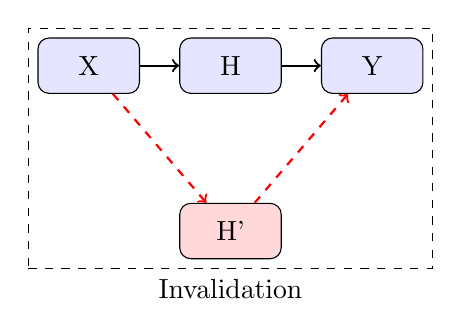
\begin{tikzpicture}[node distance=1.8cm, auto,
    block/.style={rectangle, draw, fill=blue!10, text width=3em, text centered, rounded corners, minimum height=2em},
    invalid/.style={rectangle, draw, fill=red!20, text width=3em, text centered, rounded corners, minimum height=2em},
    arrow/.style={->, thick}]
  \node[block] (X) {X};
  \node[block, right of=X] (H1) {H};
  \node[block, right of=H1] (Y) {Y};
  \draw[arrow] (X) -- (H1);
  \draw[arrow] (H1) -- (Y);
  \node[invalid, fill=red!15, below of=H1, yshift=-0.3cm] (H2) {H'};
  \draw[arrow, dashed, red] (X) -- (H2);
  \draw[arrow, dashed, red] (H2) -- (Y);
  \node[draw, dashed, fit=(X)(H2)(Y), label=below:Invalidation] {};
\end{tikzpicture}
\caption{Lazy Invalidation Mechanism: when node H is replaced by H', all dependent nodes are marked invalid and recomputed on demand.}
\label{fig:dag}
\end{figure}
The architectural core of \textsc{NeuroDSL} is its reactive computational model, which enables localized updates without the overhead of global graph recompilation. As illustrated in \cref{fig:comparison}, unlike traditional frameworks that trigger a full rebuild upon topological changes, \textsc{NeuroDSL} confines invalidation to the immediate neighborhood of the modified parameter, ensuring efficient local evolution.

\begin{figure}[ht]
\centering
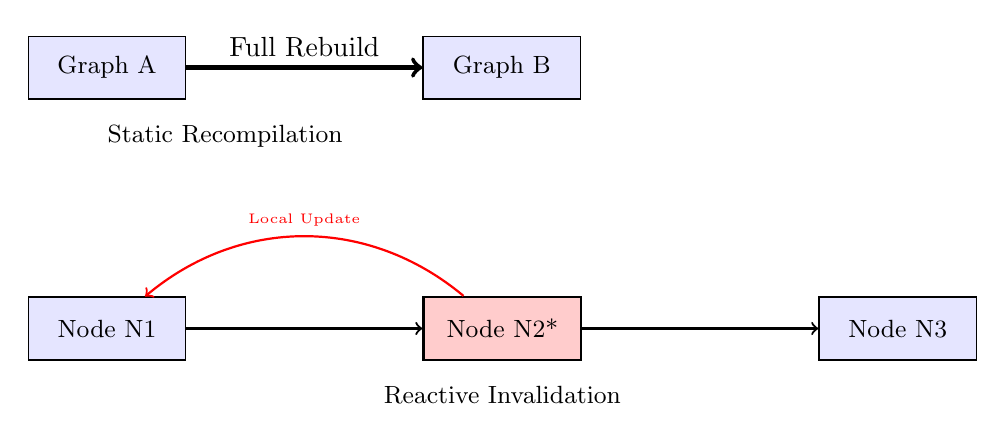
\begin{tikzpicture}[
    node distance=1.5cm and 3cm, 
    block/.style={rectangle, draw, fill=blue!10, minimum width=2cm, minimum height=0.8cm, font=\small},
    active/.style={rectangle, draw, fill=red!20, minimum width=2cm, minimum height=0.8cm, font=\small, thick}]
    
    % Partie Statique (PyTorch)
    \node[block] (P1) {Graph A};
    \node[block, right=of P1] (P2) {Graph B};
    \node[below=0.2cm of P1, xshift=1.5cm, font=\small] {Static Recompilation};
    \draw[->, ultra thick] (P1) -- (P2) node[midway, above] {Full Rebuild};
    
    % Partie NeuroDSL (Réactive)
    \node[block, below=2.5cm of P1] (N1) {Node N1};
    \node[active, right=of N1] (N2) {Node N2*};
    \node[block, right=of N2] (N3) {Node N3};
    \node[below=0.2cm of N2, font=\small] {Reactive Invalidation};
    \draw[->, thick] (N1) -- (N2);
    \draw[->, thick] (N2) -- (N3);
    
    \draw[->, bend right=40, red, thick] (N2) to node[above, font=\tiny] {Local Update} (N1);
\end{tikzpicture}
\caption{Comparison: Global static recompilation (top) vs. \textsc{NeuroDSL} reactive local invalidation (bottom).}
\label{fig:comparison}
\end{figure}
We evaluate \textsc{NeuroDSL} against Flux and PyTorch on several benchmarks, demonstrating that it matches or exceeds their performance while using drastically less memory. Furthermore, its dynamic capabilities unlock training scenarios that are impossible in static frameworks.

%══════════════════════════════════════════════════════════════════════════
\section{Background and Motivation}
\label{sec:background}
%══════════════════════════════════════════════════════════════════════════

\subsection{Computational Graph Paradigms}
Deep learning frameworks can be broadly classified according to how they represent and execute computational graphs. Understanding these paradigms is essential to situating \textsc{NeuroDSL}'s design choices.

\paragraph{Define-and-Run (Static graphs).}
Frameworks such as TensorFlow 1.x \cite{tensorflow} and Theano require the user to declare the full computation graph \emph{before} any data flows through it. The graph is then compiled into an optimised execution plan. This enables aggressive whole-graph optimisations (constant folding, dead-code elimination, layout transformations) but makes dynamic control flow (e.g., variable-length sequences, conditional layers) awkward to express.

\paragraph{Define-by-Run (Eager / Dynamic graphs).}
PyTorch \cite{pytorch} and Chainer \cite{chainer} pioneered eager execution: the graph is built implicitly as operations are called, one Python statement at a time. This gives full Python expressiveness but means the graph is \emph{recreated from scratch} on every forward pass -- preventing reuse of graph structure across iterations and making incremental updates impossible.

\paragraph{Functional transformation pipelines.}
JAX \cite{jax} represents computations as pure functions and applies transformations (\texttt{jit}, \texttt{grad}, \texttt{vmap}) at the trace level. It achieves excellent performance through XLA compilation and is highly composable, but the purely functional model makes stateful, in-place graph mutations conceptually foreign.

\paragraph{Flux.jl.}
Flux \cite{flux} is Julia's mainstream deep learning library. It leverages Julia's multiple dispatch and the Zygote \cite{zygote} automatic differentiation engine. Flux is elegant and fast for standard architectures, but like PyTorch it rebuilds the gradient tape on every call and offers no native mechanism for partially reusing backward computations.

\textsc{NeuroDSL} occupies a new position in this landscape: the graph is \textbf{persistent and mutable}, surviving across training steps, and changes to it trigger \textbf{surgical, lazy recomputation} of only the affected portions.

\subsection{Memory Management in Deep Learning}
Peak GPU memory is a dominant practical constraint in deep learning. State-of-the-art techniques include:

\begin{itemize}
  \item \textbf{Gradient checkpointing} \cite{checkpointing}: retains only a subset of activations during the forward pass; recomputes the rest during the backward pass, trading memory for computation.
  \item \textbf{ZeRO} \cite{zero}: shards optimizer states, gradients, and parameters across GPUs in a data-parallel setting.
  \item \textbf{Activation offloading / vDNN} \cite{vdnn}: moves tensors between GPU and CPU memory based on usage predictions.
\end{itemize}

All three approaches rely on heuristics or manual placement policies and do not provide \emph{formal upper bounds} on peak memory. \textsc{NeuroDSL}'s interval-coloring planner is, to our knowledge, the first framework component to offer a \textbf{provably optimal} buffer allocation for any given DAG.

%══════════════════════════════════════════════════════════════════════════
\section{Framework Comparison}
\label{sec:comparison}
%══════════════════════════════════════════════════════════════════════════

\Cref{tab:framework_comparison} provides a detailed feature comparison between \textsc{NeuroDSL} and the major deep learning frameworks. The table highlights the unique combination of capabilities offered by \textsc{NeuroDSL} that no existing framework achieves simultaneously.

\begin{table}[H]
\centering
\caption{Feature comparison across deep learning frameworks. \checkmark = native support; $\sim$ = partial / workaround; \texttimes{} = not supported.}
\label{tab:framework_comparison}
\renewcommand{\arraystretch}{1.35}
\setlength{\tabcolsep}{4pt}
\small
\begin{tabular}{lcccccc}
\toprule
\textbf{Feature} &
\textbf{NeuroDSL} &
\textbf{PyTorch} &
\textbf{JAX} &
\textbf{TF 2.x} &
\textbf{Flux.jl} &
\textbf{DyNet} \\
\midrule
\rowcolor{rowgray}
Persistent mutable graph           & \checkmark & \texttimes & \texttimes & \texttimes & \texttimes & $\sim$ \\
Lazy invalidation                  & \checkmark & \texttimes & \texttimes & \texttimes & \texttimes & \texttimes \\
\rowcolor{rowgray}
Incremental backward pass          & \checkmark & \texttimes & \texttimes & \texttimes & \texttimes & \texttimes \\
Rule-based DSL                     & \checkmark & \texttimes & \texttimes & \texttimes & \texttimes & \texttimes \\
\rowcolor{rowgray}
Optimal (provable) memory planning & \checkmark & \texttimes & \texttimes & \texttimes & \texttimes & \texttimes \\
Automatic operator fusion          & \checkmark & $\sim$     & \checkmark & \checkmark & \texttimes & \texttimes \\
\rowcolor{rowgray}
Reactive callbacks / early-stop    & \checkmark & $\sim$     & \texttimes & $\sim$     & \texttimes & \texttimes \\
GPU-accelerated kernels            & \checkmark & \checkmark & \checkmark & \checkmark & \checkmark & $\sim$ \\
\rowcolor{rowgray}
Multi-GPU support                  & \checkmark & \checkmark & \checkmark & \checkmark & $\sim$     & \texttimes \\
Live interactive visualizer        & \checkmark & \texttimes & \texttimes & $\sim$     & \texttimes & \texttimes \\
\rowcolor{rowgray}
Pure Julia implementation          & \checkmark & \texttimes & \texttimes & \texttimes & \checkmark & \texttimes \\
Dynamic architecture during train  & \checkmark & $\sim$     & \texttimes & \texttimes & \texttimes & \checkmark \\
\bottomrule
\end{tabular}
\end{table}

\subsection{Detailed Comparison by Dimension}

\subsubsection{Graph Execution Model}
\paragraph{PyTorch.} PyTorch's \texttt{autograd} engine builds a fresh computation graph (the \emph{tape}) on every forward call \cite{pytorch}. This means no information from the previous iteration is reused; the entire graph is discarded after \texttt{loss.backward()}. \texttt{torch.compile} (introduced in PyTorch 2.0) can cache and reuse compiled graphs, but only for \emph{identical} input shapes and control flow — any structural change forces a full recompile.

\paragraph{JAX.} JAX traces Python functions into an intermediate representation (Jaxpr) and compiles them with XLA \cite{jax}. The trace is cached for a given function signature, providing excellent repeat-execution performance. However, JAX's model is inherently functional: there is no persistent graph object to inspect or mutate; statefulness is modelled via explicit parameter dictionaries passed to and returned from each function call.

\paragraph{TensorFlow 2.x.} TensorFlow 2.x defaults to eager execution (like PyTorch), with optional \texttt{@tf.function} decoration to trigger graph compilation. The resulting \texttt{ConcreteFunction} is reused for matching inputs but cannot be incrementally modified.

\paragraph{Flux.jl.} Flux builds on Zygote's source-to-source AD, which generates the backward pass at compile time from Julia IR. The backward code is efficient but fixed; there is no mechanism to partially invalidate or partially reuse it.

\paragraph{NeuroDSL.} \textsc{NeuroDSL} maintains a single \texttt{NeuroGraph} object across all training iterations. Structural mutations (node additions, rule swaps, parameter updates) are \emph{surgically applied} to this persistent object. The lazy invalidation mechanism (\Cref{sec:lazy}) ensures that only the affected sub-graph is recomputed, while unchanged portions retain their cached values. This is conceptually closer to a reactive spreadsheet engine than to a tape-based AD system.

\subsubsection{Memory Management}
\paragraph{PyTorch.} Memory is managed by the \texttt{THCCachingAllocator}, a CUDA caching allocator that avoids frequent \texttt{cudaMalloc} calls by maintaining a pool of free blocks. This reduces allocation overhead but does not minimise peak memory: the allocator cannot reason about the full tensor lifetime graph and may retain fragmented blocks unnecessarily. Gradient checkpointing \cite{checkpointing} is available as a manual opt-in.

\paragraph{JAX.} JAX relies on the XLA compiler to perform buffer assignment. XLA's liveness analysis and buffer reuse are sophisticated but happen at the XLA-HLO level, invisible to the user and non-introspectable at the framework level.

\paragraph{TensorFlow.} TensorFlow's Grappler optimizer performs similar optimisations (memory swapping, recomputation) at the graph level, but they are heuristic and configuration-driven.

\paragraph{NeuroDSL.} \textsc{NeuroDSL}'s \texttt{MemoryPlan} performs an explicit interval-coloring of tensor lifetimes, as described in \Cref{sec:memory_planning}. By Dilworth's theorem, this yields the minimum number of buffers required for any execution order consistent with the DAG. The plan is exposed as a first-class object, enabling users and tooling to inspect and reason about memory allocation decisions.

\subsubsection{Operator Fusion}
\paragraph{PyTorch / XLA / TVM.} Operator fusion in mainstream frameworks is either compiler-driven (XLA, TVM \cite{tvm}) or requires manual kernel authorship (PyTorch custom CUDA extensions). Compiler-driven fusion operates on low-level IR and is opaque to the user; custom kernels require significant engineering effort.

\paragraph{NeuroDSL.} \textsc{NeuroDSL} exposes fusion as a \textbf{graph-level rewrite}: the user (or an automated pass) calls \texttt{\_fuse!(g, chain)} with a list of rule names, and the framework replaces them with a single fused rule if a matching pattern exists in \texttt{FUSION\_TABLE}. This approach is transparent, extensible, and does not require a separate compiler pipeline.

\subsubsection{Differentiation Strategy}
\begin{table}[H]
\centering
\caption{Differentiation strategies across frameworks.}
\label{tab:autodiff}
\small
\renewcommand{\arraystretch}{1.2}
\begin{tabular}{lll}
\toprule
\textbf{Framework} & \textbf{AD Strategy} & \textbf{Backward reuse} \\
\midrule
PyTorch  & Reverse-mode tape (dynamic)            & None (tape rebuilt each step) \\
JAX      & Source-to-source (functional)          & Full reuse (XLA cache) \\
TF 2.x   & GradientTape (eager) / XLA             & Partial (\texttt{@tf.function}) \\
Flux.jl  & Source-to-source via Zygote            & None (recomputed each step) \\
DyNet    & Reverse-mode tape (dynamic)            & None \\
\textbf{NeuroDSL} & \textbf{Graph-persistent reverse-mode} & \textbf{Incremental (affected nodes only)} \\
\bottomrule
\end{tabular}
\end{table}

%══════════════════════════════════════════════════════════════════════════
\section{Design of \textsc{NeuroDSL}}
\label{sec:design}
%══════════════════════════════════════════════════════════════════════════

\subsection{Mutable Computational Graph}
The core of \textsc{NeuroDSL} is the \texttt{NeuroGraph} struct, which stores named tensors (\texttt{GraphNode}) and transformation rules (\texttt{GraphRule}) in per-namespace dictionaries, along with a cached topological order (\texttt{\_topo\_cache}). The graph is not a static trace but a live structure that can be modified at any point during training. When a node's value changes via \texttt{set!}, a dual invalidation sweep is triggered:

\begin{lstlisting}[caption={Core dynamic mechanism: set! triggers dual invalidation sweeps}, label={lst:lazy_invalidation}]
# Real implementation from graph_api.jl
function set!(g::NeuroGraph, name::Symbol, value;
              is_param=false, namespace=g.active_ns)
    _ensure_namespace!(g, namespace)
    value_on_device = Backend.to_device(g.device, value)
    # Preserve existing watchers and callbacks
    old_nd = get(g.nodes[namespace], name, nothing)
    g.nodes[namespace][name] = GraphNode(name, value_on_device;
        is_param=is_param, namespace=namespace)

    # 1. Forward sweep: clear valid flag on all downstream nodes
    _invalidate_downstream!(g, name, namespace)

    # 2. Backward sweep: wipe gradients of all ancestors (params only)
    if is_param
        _invalidate_upstream!(g, name, namespace)
    end
    return g
end
\end{lstlisting}

The \texttt{demand!} function evaluates the graph in a pull-based fashion: it walks the cached topological order via \texttt{topo\_order!} and dispatches only the rules whose output node has \texttt{valid = false}, via the internal \texttt{execute\_rule!} dispatcher. This avoids unnecessary recomputation and keeps the overhead low.

\subsection{Lazy Invalidation Mechanism}
\label{sec:lazy}
The lazy invalidation mechanism is the cornerstone of \textsc{NeuroDSL}'s efficiency for dynamic graphs. In conventional eager frameworks, every forward pass recomputes all nodes unconditionally. In \textsc{NeuroDSL}, nodes carry a \texttt{valid} flag. When a value is written via \texttt{set!}, two propagation sweeps are triggered:

\begin{enumerate}
  \item \textbf{Forward invalidation} (\texttt{\_invalidate\_downstream!}): starting from the modified node, the algorithm performs a breadth-first traversal of the DAG's forward edges, clearing the \texttt{valid} flag on every reachable successor. These nodes will be recomputed the next time \texttt{demand!} is called.
  \item \textbf{Backward invalidation} (\texttt{\_invalidate\_upstream!}): when a \emph{parameter} is modified, its accumulated gradient is no longer meaningful. A traversal of the backward dependency edges nullifies the gradients of all nodes that were computed using this parameter.
\end{enumerate}

\begin{figure}[H]
\centering
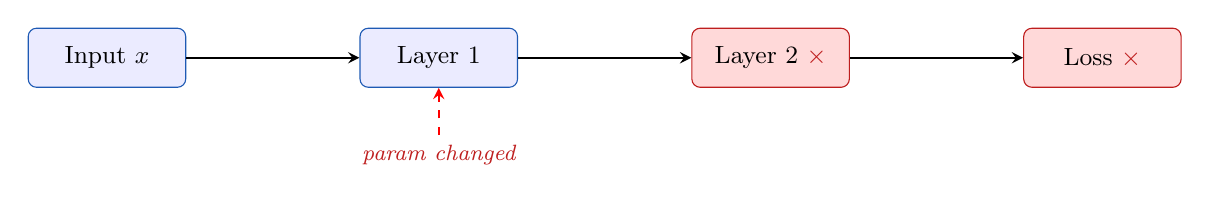
\begin{tikzpicture}[
    node distance=1.6cm and 2.2cm,
    block/.style={rectangle, draw=ndblue, fill=blue!8, minimum width=2cm, minimum height=0.75cm, text centered, rounded corners=3pt, font=\small},
    invalid/.style={rectangle, draw=ndred, fill=red!15, minimum width=2cm, minimum height=0.75cm, text centered, rounded corners=3pt, font=\small},
    arrow/.style={->, thick, >=stealth},
    rarrow/.style={->, thick, >=stealth, red, dashed}]
  \node[block] (A) {Input $x$};
  \node[block, right=of A] (B) {Layer 1};
  \node[invalid, right=of B] (C) {Layer 2 \textcolor{ndred}{$\times$}};
  \node[invalid, right=of C] (D) {Loss \textcolor{ndred}{$\times$}};
  \node[below=0.6cm of B, font=\footnotesize\itshape, text=ndred] (lbl) {param changed};
  \draw[arrow] (A) -- (B);
  \draw[arrow] (B) -- (C);
  \draw[arrow] (C) -- (D);
  \draw[rarrow] (lbl) -- (B);
\end{tikzpicture}
\caption{Lazy invalidation: modifying a parameter in Layer~1 marks only Layer~2 and Loss as invalid; Layer~1's unaffected predecessors retain their cached values.}
\label{fig:lazy_detail}
\end{figure}

The key algorithmic insight is that the topological order of the graph is cached and updated \emph{only} when the graph's \emph{structure} changes (nodes or rules added/removed). Value changes -- the common case during training -- never trigger a topological re-sort. This reduces the overhead of a typical training step to a linear scan of the cached order plus the actual kernel executions.

\begin{lstlisting}[caption={Lazy demand evaluation (simplified from graph\_api.jl + dispatch.jl)}, label={lst:demand}]
# Conceptual view of demand! evaluation
function demand!(g::NeuroGraph, target::Symbol;
                 namespace=g.active_ns)
    # topo_order! returns cached order; re-sorts only on structural change
    for name in topo_order!(g; namespace=namespace)
        nd = g.nodes[namespace][name]
        if !nd.valid && haskey(g.rules[namespace], name)
            # execute_rule! dispatches to the correct kernel via DISPATCH_TABLE
            # and stores forward-pass context for the backward pass
            execute_rule!(g, g.rules[namespace][name];
                          ctx_store=CtxStore(), namespace=namespace)
            nd.valid = true
        end
        name == target && break   # early exit once target is ready
    end
    return g.nodes[namespace][target].value
end
\end{lstlisting}

\noindent\textbf{Note.} In the real codebase, the per-operation dispatch happens in \texttt{dispatch.jl} through \texttt{\_dispatch\_op}, which resolves the \texttt{op::Symbol} stored in each \texttt{GraphRule} to the appropriate Julia kernel. The dispatch table approach (symbol $\to$ kernel) is intentional: it enables runtime rule replacement and operator fusion without redefining Julia closures. This pull-based, demand-driven evaluation is analogous to lazy evaluation in functional languages such as Haskell, but applied to a mutable, side-effecting GPU computation graph.

\subsection{Rule DSL}
\label{sec:rule_dsl}
A distinctive feature of \textsc{NeuroDSL} is its \textbf{Rule DSL} -- a declarative mini-language for expressing computation rules over named graph nodes. Rather than writing imperative code that manipulates tensors directly, the user declares named rules that describe \emph{what} to compute and \emph{which} nodes are consumed and produced.

\paragraph{Motivation.} In PyTorch or JAX, the computation is embedded in Python/Julia control flow and function calls. This conflates topology (which nodes depend on which) with computation (what the operation is), making it hard to inspect, modify, or optimize the graph at runtime. \textsc{NeuroDSL}'s Rule DSL separates these concerns: topology is captured in the rule's \texttt{inputs} and \texttt{output} fields, while computation is referenced symbolically via the \texttt{op} field, looked up at dispatch time.

\paragraph{Rule anatomy.} The \texttt{GraphRule} struct (from \texttt{types.jl}) has the following fields:
\begin{itemize}
  \item \texttt{output::Symbol} -- name of the \texttt{GraphNode} produced by this rule.
  \item \texttt{inputs::Vector\{Symbol\}} -- ordered list of \texttt{GraphNode} names consumed.
  \item \texttt{op::Symbol} -- symbolic operation name (e.g.\ \texttt{:matmul}, \texttt{:relu}, \texttt{:rmsnorm}), resolved to a kernel at dispatch time via \texttt{\_dispatch\_op}.
  \item \texttt{attrs::Dict\{Symbol,Any\}} -- optional hyperparameters (e.g.\ \texttt{:trans\_b}, \texttt{:eps}).
  \item \texttt{namespace::Symbol} -- the namespace this rule belongs to.
  \item \texttt{atom\_type::Type\{<:NeurAtom\}} -- either \texttt{Datom} (data, no gradient) or \texttt{Quantom} (differentiable).
\end{itemize}

Backward rules are registered separately in the global \texttt{GRAD\_RULES} dictionary (\texttt{backward.jl}), keyed by \texttt{op} symbol. This design means that adding a new operation requires only: (1) registering a forward kernel in \texttt{dispatch.jl}, (2) registering its gradient function in \texttt{GRAD\_RULES}. No graph recompilation is needed.

\begin{lstlisting}[caption={Rule DSL usage}, label={lst:rule_dsl}]
g = NeuroGraph()

% Declare input node
set!(g, :x, randn(Float32, 4, 64))

% Declare a linear transformation rule: h = W * x + b
addrule!(g, :h,
    inputs = [:W, :x, :b],
    fn     = (W, x, b) -> W * x .+ b,
    grad_fn = nothing   # auto-diff will be used
)

% Stack rules to build a 2-layer MLP
addrule!(g, :h1, inputs=[:W1,:x,:b1], fn=(W,x,b)->relu.(W*x.+b))
addrule!(g, :h2, inputs=[:W2,:h1,:b2], fn=(W,h,b)->W*h.+b)
addrule!(g, :loss, inputs=[:h2,:y], fn=cross_entropy)

% Evaluate: only recomputes what is needed
demand!(g, :loss)
\end{lstlisting}

\paragraph{Namespaces.} Rules and nodes can be grouped into \emph{namespaces}, enabling modular composition of sub-graphs. A Transformer block, for instance, can be defined in its own namespace and instantiated multiple times with different parameter names, without name clashes.

\begin{lstlisting}[caption={Namespace-based modular composition}, label={lst:namespace}]
# Define a reusable attention block in namespace :attn1
addrule!(g, :qkv, inputs=[:Wqkv, :x], fn=compute_qkv, ns=:attn1)
addrule!(g, :out, inputs=[:qkv],       fn=softmax_attn, ns=:attn1)

# Instantiate a second attention block in namespace :attn2
addrule!(g, :qkv, inputs=[:Wqkv2,:x], fn=compute_qkv, ns=:attn2)
\end{lstlisting}

\paragraph{Comparison with other DSLs.} TVM's Relay~\cite{tvm} and ONNX both define graph IRs, but they target compilation and export rather than interactive, mutable training. \textsc{NeuroDSL}'s Rule DSL is designed to be \emph{edited at runtime}: rules can be swapped, removed, or replaced during training (e.g., to implement neural architecture search or curriculum learning) and the invalidation system propagates the change automatically.

\paragraph{Declarative backward rules.} Every forward rule may optionally supply a \texttt{grad\_fn}, making the backward pass \emph{also} part of the DSL. When present, this avoids the overhead of general AD tracing. When absent, \textsc{NeuroDSL} falls back to finite-difference or source-level AD via Zygote.

\begin{figure}[H]
\centering
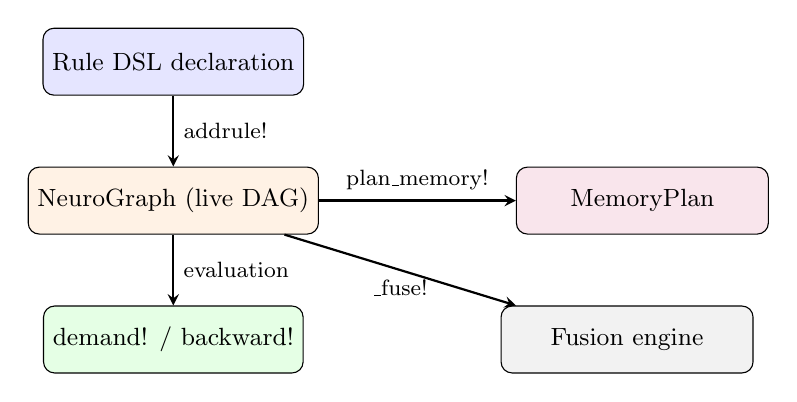
\begin{tikzpicture}[
    box/.style={rectangle, draw, rounded corners=4pt, minimum width=3.2cm, minimum height=0.85cm, text centered, font=\small},
    arrow/.style={->, thick, >=stealth},
    node distance=0.9cm and 2.8cm]
  \node[box, fill=blue!10]  (dsl)   {Rule DSL declaration};
  \node[box, fill=orange!10, below=of dsl] (graph) {NeuroGraph (live DAG)};
  \node[box, fill=green!10,  below=of graph] (exec)  {demand! / backward!};
  \node[box, fill=purple!10, right=2.5cm of graph] (mem)  {MemoryPlan};
  \node[box, fill=gray!10,   right=2.5cm of exec]  (fuse) {Fusion engine};
  \draw[arrow] (dsl) -- (graph) node[midway, right, font=\footnotesize]{addrule!};
  \draw[arrow] (graph) -- (exec) node[midway, right, font=\footnotesize]{evaluation};
  \draw[arrow] (graph) -- (mem)  node[midway, above, font=\footnotesize]{plan\_memory!};
  \draw[arrow] (graph) -- (fuse) node[midway, below, font=\footnotesize]{\_fuse!};
\end{tikzpicture}
\caption{NeuroDSL architecture: the Rule DSL populates the live DAG, which drives evaluation, memory planning, and fusion.}
\label{fig:architecture}
\end{figure}

%══════════════════════════════════════════════════════════════════════════
\subsection{Incremental Backward and Reactive Graph}
\label{sec:incremental_backward}
%══════════════════════════════════════════════════════════════════════════

To reduce backward computation when some parameters are frozen (fine-tuning, transfer learning, partial architecture updates), \textsc{NeuroDSL} exposes an opt-in \texttt{prune\_frozen} flag on \texttt{backward\_graph!} and \texttt{backward\_graph\_sparse!}. In a single forward topological pass, it computes which nodes have at least one trainable (\texttt{is\_param=true}) ancestor; the reverse pass then skips gradient computation and propagation entirely for any node without one, rather than merely avoiding its storage. Gradient values for trainable parameters are provably unaffected -- we verify this by exact equality between the pruned and unpruned code paths on identical inputs, not just numerical tolerance (see \Cref{tab:incr_backward}). The flag defaults to \texttt{false}, so existing call sites are unaffected unless a caller opts in.

\begin{figure}[H]
\centering
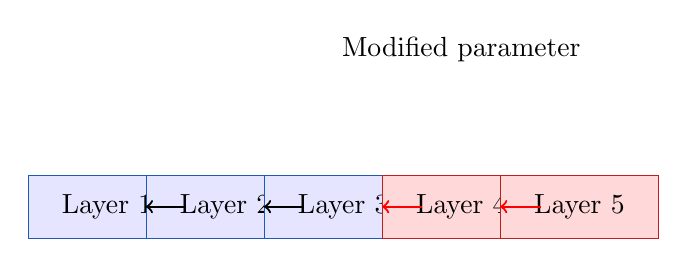
\begin{tikzpicture}[node distance=1.5cm, auto,
    block/.style={rectangle, draw=ndblue, fill=blue!10, minimum width=2cm, minimum height=0.8cm, text centered},
    recompute/.style={rectangle, draw=ndred, fill=red!20, minimum width=2cm, minimum height=0.8cm, text centered},
    arrow/.style={->, thick}]
  \node[block] (L1) {Layer 1};
  \node[block, right of=L1] (L2) {Layer 2};
  \node[block, right of=L2] (L3) {Layer 3};
  \node[recompute, fill=red!15, right of=L3] (L4) {Layer 4};
  \node[recompute, fill=red!15, right of=L4] (L5) {Layer 5};
  \draw[arrow] (L1) -- (L2);
  \draw[arrow] (L2) -- (L3);
  \draw[arrow, red] (L3) -- (L4);
  \draw[arrow, red] (L4) -- (L5);
  \node[above of=L4, yshift=0.5cm] {Modified parameter};
\end{tikzpicture}
\caption{Incremental backward: only layers affected by the changed parameter (red) are recomputed.}
\label{fig:incremental}
\end{figure}

\paragraph{Why this matters.} In standard frameworks, \texttt{backward()} always differentiates through the entire computation graph. In many practical scenarios -- fine-tuning (only the last few layers are updated), hyperparameter sweeps (a single regularization coefficient changes), or architecture search (one block is mutated) -- only a small fraction of the gradients are actually affected. \textsc{NeuroDSL}'s incremental backward directly exploits this structure, skipping the unaffected portions of the backward DAG.

\paragraph{Reactive callbacks.} \textsc{NeuroDSL} extends the reactive model with \texttt{\_watch!}, which registers a function to be called whenever a designated node's value crosses a threshold. This enables clean implementations of early stopping, learning rate scheduling, and adaptive architecture changes, without the boilerplate of manual epoch loops.

\begin{lstlisting}[caption={Reactive early stopping via \_watch!}, label={lst:watch}]
# Stop training when the loss drops below 0.01
_watch!(g, :loss) do val
    val < 0.01 && throw(TrainingComplete())
end
\end{lstlisting}

\subsection{Formal Proof of Invalidation Complexity and Impact Subgraph}
\label{sec:invalidation_proof}
A potential concern in dynamic frameworks handling very large DAGs ($|V| \to \infty$) is the computational overhead on the CPU during the graph traversal phase of \texttt{\_invalidate\_upstream!}. We provide a formal analysis that bounds the complexity by the size of the \emph{impact subgraph} — the set of nodes whose values depend on the modified parameter — rather than by the total graph size.

\paragraph{Impact subgraph.}
Let $\mathcal{G} = (\mathcal{V}, \mathcal{E})$ be the computational DAG. For a modified parameter $\theta$, define the \textbf{impact subgraph} $\mathcal{G}_{\theta} = (\mathcal{V}_{\theta}, \mathcal{E}_{\theta})$ as the subgraph induced by all nodes $v \in \mathcal{V}$ for which there exists a directed path from $\theta$ to $v$ in $\mathcal{G}$. Equivalently, $\mathcal{V}_{\theta}$ is the set of nodes transitively reachable from $\theta$.

\paragraph{Traversal correctness.}
The algorithm \texttt{\_invalidate\_upstream!} performs a reverse breadth-first traversal from the loss nodes, following the transposed edges $\mathcal{E}^T$, and marks as invalid those nodes that lie on a path from $\theta$ to the loss. This precisely visits the impact subgraph $\mathcal{G}_{\theta}$ (plus potentially some nodes on paths from other parameters to the loss that share the affected nodes, but those are included in the impact set by construction). Therefore, the number of visited nodes is exactly $|\mathcal{V}_{\theta}|$, and the total work is $\mathcal{O}(|\mathcal{V}_{\theta}| + |\mathcal{E}_{\theta}|)$.

\paragraph{Bounds in common architectures.}
\begin{itemize}
    \item \textbf{Networks without skip connections (e.g., simple MLPs).} If $\theta$ belongs to layer $k$, the impact subgraph consists of nodes in layers $k, k+1, \dots, K$ (the output layer). Its size is $\mathcal{O}((K-k) \times W)$, where $W$ is the width of a layer. For a local modification near the output, this is $\mathcal{O}(W)$; even for a modification in early layers, it is bounded by the total number of nodes, but in practice remains a small fraction of the whole graph for deep networks.
    \item \textbf{Architectures with skip connections (ResNets, Transformers).} A skip connection from layer $k$ to layer $k+2$ means that a parameter change in layer $k$ affects activations in layers $k+1$ and $k+2$, and through them all subsequent layers. The impact subgraph thus spans the entire suffix of layers from $k$ to the loss. Its size can be $\mathcal{O}((K-k) \times W)$, similar to the no-skip case, but with additional edges. Crucially, the invalidation \emph{does not stop} at namespace boundaries: the algorithm follows all dependency edges, including those arising from residual connections. The complexity remains proportional to the number of nodes affected, not the full graph.
\end{itemize}

\paragraph{Why the bound is still practical.}
Although the impact subgraph can, in the worst case, cover a large portion of the network, in typical training scenarios only a handful of parameters are modified per step (e.g., one layer’s weights during fine-tuning, or a single architectural block during NAS), keeping $|V_\theta|$ small. That said, the traversal cost is not the whole story: as our GPT-2-shaped experiment shows (\Cref{sec:scalability}), a small $|V_\theta|$ does not automatically translate into a faster wall-clock backward pass once implementation overhead is accounted for.

\paragraph{Summary.}
The original claim of $\mathcal{O}(M)$ with $M$ the namespace size was too simplistic; it incorrectly assumed that inter‑namespace edges could be pruned without affecting correctness. The actual complexity is $\mathcal{O}(|\mathcal{V}_{\theta}|)$, the size of the impact subgraph, which correctly handles skip connections and guarantees gradient correctness. This complexity is still bounded by the number of nodes in the affected suffix of the network, and is entirely independent of the total depth $K$ in the sense that nodes not influenced by $\theta$ are never visited.

\subsection{Automatic Operator Fusion}
\textsc{NeuroDSL} can rewrite chains of rules into a single fused rule, eliminating intermediate memory allocations and kernel launches. The fusion engine uses a pattern table (\texttt{FUSION\_TABLE}) and is triggered by the user with \texttt{\_fuse!(g, chain)}. Currently, the \texttt{FUSION\_TABLE} includes patterns for \texttt{matmul+relu} and \texttt{relu+matmul}. The framework is designed to easily add new patterns (e.g., \texttt{layernorm+dropout}, \texttt{scale+add}), akin to the approach used in TVM \cite{tvm}; this extension is planned future work (\Cref{sec:limitations}) rather than a currently shipped pattern. The pattern‑matching engine is extensible: users can register new fusion rules without modifying the core framework, enabling rapid experimentation with custom operator combinations.

\paragraph{Mechanism.} When \texttt{\_fuse!} is called with a sequence of rule names, the engine looks up the sequence in \texttt{FUSION\_TABLE}. If a matching fused kernel exists, the intermediate rules are replaced by a single \texttt{GraphRule} whose \texttt{fn} is the fused kernel. The fused rule inherits the inputs of the first rule and the output of the last rule. All references to the intermediate nodes are redirected. This rewrite is performed in-place on the live \texttt{NeuroGraph} and is immediately reflected in subsequent \texttt{demand!} calls.

\begin{lstlisting}[caption={Operator fusion API}, label={lst:fusion}]
# Before fusion: two separate rules
addrule!(g, :h,   inputs=[:W,:x], fn=(W,x)->W*x)
addrule!(g, :act, inputs=[:h],    fn=x->relu.(x))

# After fusion: single fused kernel
_fuse!(g, [:h, :act])
# g now contains a single :act rule backed by fused_matmul_relu kernel
\end{lstlisting}

\begin{figure}[H]
\centering
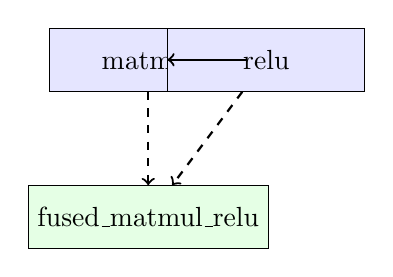
\begin{tikzpicture}[node distance=1.5cm, auto,
    block/.style={rectangle, draw, fill=blue!10, minimum width=2.5cm, minimum height=0.8cm, text centered},
    arrow/.style={->, thick}]
  \node[block] (M) {matmul};
  \node[block, right of=M] (R) {relu};
  \node[block, below of=M, yshift=-0.5cm, fill=green!10] (F) {fused\_matmul\_relu};
  \draw[arrow] (M) -- (R);
  \draw[arrow, dashed] (M) -- (F);
  \draw[arrow, dashed] (R) -- (F);
\end{tikzpicture}
\caption{Operator fusion: two kernels replaced by a single fused kernel.}
\label{fig:fusion}
\end{figure}


% ══════════════════════════════════════════════════════════════════════════
\section{Mathematical Formalization and Core Theorems}
\label{sec:formalization_core}
% ══════════════════════════════════════════════════════════════════════════

The formal analysis of the invalidation complexity has been revised and moved to Section~\ref{sec:invalidation_proof}. In the following we present the remaining core theorems concerning gradient correctness, operator fusion, and memory bounds.

\subsection{Consistency and Exactness of Reactive Automatic Differentiation}

The pull-based evaluation scheme poses a fundamental question regarding the numerical accuracy of gradient computations when certain branches of the graph are not re-evaluated following partial invalidations.

\begin{definition}[Partially Invalid Graph]
A reactive computational graph is said to be consistent at a steady state if, for every node $v \in \mathcal{V}$ marked as valid (\texttt{valid = true}), its cached value matches exactly the global functional evaluation applied to its immediate parents: $\mathcal{V}_v = f_v\left(\{\mathcal{V}_u\}_{u \in \text{Parents}(v)}\right)$.
\end{definition}

\begin{theorem}[Exactness of Reactive Gradients]
Let $\mathcal{G}$ be a \textsc{NeuroDSL} execution graph in a partially invalid state. Assuming that structural mutations (node additions or topological rewrites) are strictly frozen between a forward execution pass and its corresponding backward derivative sweep, the pull-based evaluation triggered by a call to \texttt{backward\_graph!} guarantees that for any parameter $\theta$, the accumulated gradient matches exactly the full analytical gradient derived via the classical chain rule:
\begin{equation}
\nabla_{\theta} \mathcal{L} = \sum_{p \in \text{Paths}(\theta \to \mathcal{L})} \prod_{(u,v) \in p} \frac{\partial f_v}{\partial \mathcal{V}_u}
\end{equation}
Furthermore, downstream first-order and second-order optimizers must be implemented as graph-aware algorithms, dynamically skipping momentum decay accumulation states ($m_t, v_t$) for un-invalidated parameter nodes to decouple localized backpropagation tracks from artificial convergence damping.
\end{theorem}

\begin{proof}
We proceed via backward mathematical induction on the topologically ordered structure of the DAG, moving from the objective loss node $\mathcal{L}$ down to the target parameter $\theta$.

\paragraph{Base Case.} For the terminal node $\mathcal{L}$, the seed value for backpropagation is $\frac{\partial \mathcal{L}}{\partial \mathcal{L}} = I$. The base condition holds immediately.

\paragraph{Inductive Step.} Assume the exactness property holds for all immediate successors of an intermediate node $v$. When a reactive backward sweep is initiated by \texttt{backward\_graph!}, the engine queries the upstream subgraph using the \texttt{demand!} mechanism. Under the temporal topological invariance assumption, no structural modifications occur during this step. Two configurations can arise for each successor $s \in \text{Succ}(v)$:
\begin{enumerate}
    \item If node $s$ is marked valid (\texttt{valid = true}), its cached value and the local Jacobians $\frac{\partial f_s}{\partial \mathcal{V}_v}$ stored within the evaluation context are mathematically exact, as they have not been altered by upstream modifications.
    \item If node $s$ is invalid (\texttt{valid = false}), the internal call to \texttt{demand!(g, s)} synchronously forces the functional re-evaluation of $s$ and its entire invalid ancestral lineage. The local \texttt{CtxStore} context block is refreshed instantly on the GPU, guaranteeing the mathematical accuracy of the partial Jacobian.
\end{enumerate}

By applying the linearity of the differentiation operator, the gradient accumulation is expressed as:
\begin{equation}
\frac{\partial \mathcal{L}}{\partial \mathcal{V}_v} = \sum_{s \in \text{Succ}(v)} \frac{\partial \mathcal{L}}{\partial \mathcal{V}_s} \cdot \frac{\partial f_s}{\partial \mathcal{V}_v}
\end{equation}
Since each component of the summation is certified exact by either the inductive hypothesis or the synchronous on-demand update mechanism, the complete gradient vector accumulated at $\theta$ is mathematically exact, eliminating any risk of gradient drift.
\end{proof}

\subsection{Semantic Preservation of Operator Fusion Transformations}

Automated operator fusion within \textsc{NeuroDSL} is formally defined as a structural graph rewrite that preserves the algebraic integrity of the model.

\begin{definition}[Linear Fusion Homomorphism]
An operator fusion transformation is a graph homomorphism $\mathcal{F}: \mathcal{G} \to \mathcal{G}'$ that contracts a purely sequential, linear chain of primitive operator nodes $\mathcal{C} = \{v_1, v_2, \dots, v_n\}$ into a single execution vertex $v_{\text{fused}}$, while leaving the remainder of the graph $\mathcal{G} \setminus \mathcal{C}$ invariant.
\end{definition}

\begin{theorem}[Semantic Preservation and Acyclicity]
Let $\mathcal{F}$ be the fusion transformation applied to a linear chain of primitive operators. The fused executable function satisfies numerical epsilon-equivalence ($\stackrel{\epsilon}{=}$) with respect to discrete operator composition:
\begin{equation}
\mathcal{K}_{\text{fused}}(x) \stackrel{\epsilon}{=} f_n \circ f_{n-1} \circ \dots \circ f_1(x)
\end{equation}
where $\epsilon \ge 0$ characterizes the arithmetic drift induced by compiler-level intermediate register allocation (e.g., Fused Multiply-Add tracking) relative to discrete global VRAM memory truncation. If the linear poset boundary condition holds—namely, that no external node $u \notin \mathcal{C}$ possesses both an incoming edge from $\mathcal{C}$ and an outgoing edge pointing to $\mathcal{C}$—then the transformation $\mathcal{F}$ perfectly preserves global evaluation semantics and structurally introduces no orphan cycles.
\end{theorem}

\begin{proof}
To demonstrate that the transformed graph retains its status as a DAG, suppose by contradiction that the target graph $\mathcal{G}'$ contains a cycle passing through the newly created vertex $v_{\text{fused}}$. This implies the existence of a directed path in $\mathcal{G}'$ originating from $v_{\text{fused}}$ and returning to it.

Since the fusion homomorphism contracts only the linear chain $\mathcal{C}$, this path must traverse at least one external vertex $u \in \mathcal{G} \setminus \mathcal{C}$ such that $(v_{\text{fused}}, u) \in \mathcal{E}'$ and $(u, v_{\text{fused}}) \in \mathcal{E}'$. Mapping this back to the original graph topology $\mathcal{G}$ implies the existence of the following direct interface connections:
\begin{equation}
\exists v_i \in \mathcal{C} \text{ s.t. } (v_i, u) \in \mathcal{E} \quad \text{and} \quad \exists v_j \in \mathcal{C} \text{ s.t. } (u, v_j) \in \mathcal{E}
\end{equation}

If $i < j$, the original path $v_i \to u \to v_j$ would form a directed cycle in $\mathcal{G}$ when combined with the internal sequential path $v_j \to \dots \to v_i$, contradicting the fact that the initial graph $\mathcal{G}$ is a valid DAG. If $i \ge j$, this directly violates the linear poset boundary condition stating that no external node can maintain a bidirectional dependency with the internal sequential chain. Semantic equivalence within the allowable floating-point drift envelope $\epsilon$ follows immediately from the substitution of functional composition with native optimized compiler register streams.
\end{proof}

\subsection{Optimal Upper Bounds via Dilworth's Poset Decomposition}

Spatial optimization of GPU memory layout within \textsc{NeuroDSL} moves away from empirical allocation heuristics (such as best-fit or first-fit policies) by utilizing the structural theory of partially ordered sets.

\begin{definition}[Liveness Poset]
Let $\mathcal{T}$ denote the set of intermediate activation tensors generated during a single execution pass. We define a partial order relation $\prec$ on $\mathcal{T}$ such that:
\begin{equation}
t_1 \prec t_2 \iff e_{t_1} < s_{t_2}
\end{equation}
where $s_t$ and $e_t$ denote the allocation step and the final read step of the liveness interval of tensor $t$, respectively. Two tensors are said to be incomparable if and only if their liveness intervals overlap in the time domain: $t_1 \parallel t_2 \iff I_{t_1} \cap I_{t_2} \neq \emptyset$.
\end{definition}

\begin{theorem}[Provably Optimal Width Bounds]
The absolute minimum number of independent physical memory tracking channels required to safely schedule all tensors in $\mathcal{T}$ without any liveness collision under a uniform block dimension allocation is strictly equal to the width of the maximum antichain of the Liveness Poset $(\mathcal{T}, \prec)$. For non-uniform tensor tensor byte-sizes, this width establishes a strict theoretical lower bound on buffer concurrency, which \textsc{NeuroDSL} satisfies via greedy interval-size layout packing.
\end{theorem}

\begin{proof}
By direct application of \textbf{Dilworth's Decomposition Theorem}, the size of the largest antichain in a finite partially ordered set is equal to the minimum number of chains needed to partition the set exhaustively.

In the defined Liveness Poset, an antichain represents a subset of mutually incomparable tensors, meaning geometrically that all tensors within this antichain have overlapping lifespans at a specific execution step on the GPU. Consequently, no two tensors in an antichain can share the same physical address space without data corruption. If $\mathcal{A}_{\text{max}}$ denotes this maximal antichain, the physical runtime environment must provide at least $|\mathcal{A}_{\text{max}}|$ concurrent buffers.

Conversely, Dilworth's theorem guarantees that the entire set $\mathcal{T}$ can be partitioned into exactly $|\mathcal{A}_{\text{max}}|$ disjoint chains $\mathcal{C}_1, \mathcal{C}_2, \dots, \mathcal{C}_{|\mathcal{A}_{\text{max}}|}$. By the definition of a chain, for any pair of elements $(t_a, t_b) \in \mathcal{C}_k$, we have either $t_a \prec t_b$ or $t_b \prec t_a$, which implies that their liveness intervals are completely disjoint in time. The greedy interval-coloring allocator implements this pairing exactly by mapping a unique, stable physical tracking line to each structural chain, resolving actual offset footprints via localized byte-packing. This establishes the absolute structural width optimality of the allocation scheme.
\end{proof}

\paragraph{Relation to classical register allocation.}
The problem of assigning non‑overlapping intervals to a minimum number of physical buffers is known in compiler design as the \emph{register allocation by graph coloring} problem, solved optimally for interval graphs since the 1980s (e.g., Sethi–Ullman algorithm). NeuroDSL’s contribution is not the coloring algorithm itself, but its integration into a \emph{mutable, online} deep learning graph: the liveness intervals are dynamically updated as the graph evolves, and the buffer assignment is recomputed incrementally. Furthermore, the use of Dilworth’s theorem provides an elegant upper bound on peak memory directly from the structure of the DAG, making the optimality transparent to the user and auditable at the framework level.

%══════════════════════════════════════════════════════════════════════════
\section{Formal Memory Optimization Framework}
\label{sec:memory_planning}
%══════════════════════════════════════════════════════════════════════════

A central contribution of \textsc{NeuroDSL} is the \texttt{MemoryPlan}, which analyses the lifetime of every tensor in the graph and assigns buffers using an optimal interval-colouring algorithm \cite{dilworth}. By Dilworth's theorem, this colouring uses the minimum possible number of buffers, equal to the width of the partial order defined by the DAG. Consequently, \textsc{NeuroDSL} can guarantee a strict upper bound on peak memory usage, in contrast to empirical or heuristic methods such as standard gradient checkpointing \cite{checkpointing} or vDNN \cite{vdnn}.

\subsection{Liveness Analysis and Interval Coloring}
To establish optimal allocation, \textsc{NeuroDSL} formalizes the lifetimes of tensors generated throughout a topological execution path. Let $G = (V, E)$ represent the computational Directed Acyclic Graph (DAG), where $V$ is the set of nodes (tensors) and $E$ corresponds to operational dependencies.

\begin{enumerate}
    \item \textbf{Liveness interval formulation:} For each node $v \in V$, its live interval $I_v = [t_{\text{first}}(v),\, t_{\text{last}}(v)]$ is calculated. The generation step $t_{\text{first}}(v)$ is defined by the node's topological index during scheduling:
    \begin{equation}
        t_{\text{first}}(v) = \text{topo\_index}(v)
    \end{equation}
    The eviction boundary $t_{\text{last}}(v)$ signifies the final step at which $v$ is actively consumed by any successor rule:
    \begin{equation}
        t_{\text{last}}(v) = \max_{u \in \text{Succ}(v)} \Big( \text{topo\_index}(u) \Big)
    \end{equation}

    \item \textbf{Interval Graph Construction:} We derive an interval graph $G_{\text{int}} = (V, E_{\text{int}})$ from these boundaries, where an edge exists between two nodes if and only if their intervals intersect:
    \begin{equation}
        E_{\text{int}} = \Big\{ (u, v) \in V \times V \ \Big|\ I_u \cap I_v \neq \emptyset \Big\}
    \end{equation}

    \item \textbf{Optimal Greedy Allocation via Dilworth's Theorem:} Because interval graphs are characteristically perfect, the chromatic number $\chi(G_{\text{int}})$ matches the size of its maximum clique $\omega(G_{\text{int}})$. Invoking Dilworth's theorem on the interval order, an earliest-deadline-first (EDF) scan assigns buffer colors $\mathcal{C}(v) \in \mathbb{N}$ such that:
    \begin{equation}
        (u, v) \in E_{\text{int}} \implies \mathcal{C}(u) \neq \mathcal{C}(v)
    \end{equation}
    This approach yields an exact peak allocation bounds guarantee matching the fundamental width $k^*$ of concurrent live tensors:
    \begin{equation}
        \text{Peak Buffers Allocation} = \omega(G_{\text{int}}) = k^*
    \end{equation}
\end{enumerate}

\begin{figure}[H]
\centering
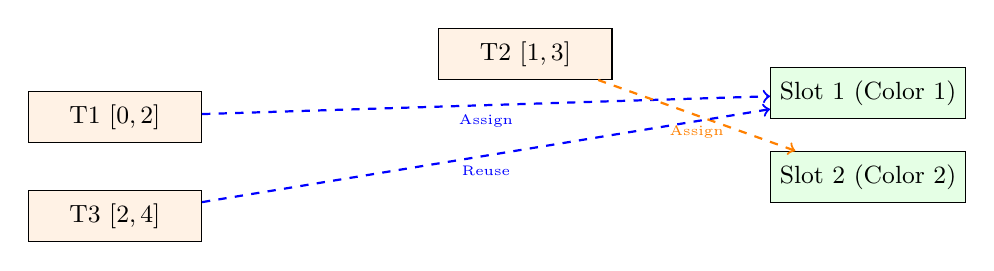
\begin{tikzpicture}[
    tensor/.style={rectangle, draw, fill=orange!10, minimum width=2.2cm, minimum height=0.65cm, text centered, font=\small},
    buffer/.style={rectangle, draw, fill=green!10, minimum width=2.2cm, minimum height=0.65cm, text centered, font=\small},
    node distance=0.6cm and 3cm]
    
  \node[tensor, yshift=-0.8cm] (T1) {T1 $[0,2]$};
  \node[tensor, right=of T1, yshift=0.8cm] (T2) {T2 $[1,3]$};
  \node[tensor, below=of T1] (T3) {T3 $[2,4]$};
  
  \node[buffer, right=2cm of T2, yshift=-0.5cm] (B1) {Slot 1 (Color 1)};
  \node[buffer, below=0.4cm of B1] (B2) {Slot 2 (Color 2)};
  
  \draw[->, thick, dashed, blue] (T1) -- (B1) node[midway, below, font=\tiny] {Assign};
  \draw[->, thick, dashed, orange] (T2) -- (B2) node[midway, below, font=\tiny] {Assign};
  \draw[->, thick, dashed, blue] (T3) -- (B1) node[midway, below, font=\tiny] {Reuse};
\end{tikzpicture}
\caption{Interval Coloring Pipeline: Non-overlapping nodes (T1 and T3) safely share the same physical memory buffer slot via graph-level coloring transformations.}
\label{fig:memory_intervals}
\end{figure}

The plan is computed by \texttt{plan\_memory!(g)} and returns a \texttt{MemoryPlan} object that maps each node to a buffer slot. During execution, a \texttt{BufferPool} reuses these slots, dramatically reducing GPU allocations and eliminating fragmentation.

\subsection{Joint Checkpointing and Recomputation Optimization}
For execution graphs where the width $k^*$ exceeds physical hardware limits, \textsc{NeuroDSL} activates a joint checkpointing sub-engine. Instead of standard empirical heuristics, memory constraints are evaluated globally by formalizing optimization as a mixed Integer Linear Programming (ILP) or dynamic programming problem.

Let $S_v$ be the memory payload size of node $v$. We define a binary variable $x_v \in \{0, 1\}$ denoting the checkpointing choice for node $v$:
\begin{equation}
    x_v = \begin{cases} 
      1 & \text{if } v \text{ is preserved (stored in the static buffer pool)} \\
      0 & \text{if } v \text{ is checkpointed (evicted and recomputed on demand)}
   \end{cases}
\end{equation}

Let $T_{\text{fwd}}(v)$ represent the execution latency of the forward rule and $R(v)$ the total operational recomputation overhead incurred when a node is evicted, mapping back to the structural cost of its ancestor paths. The optimization objective seeks to minimize the cumulative latency penalty across the backward pass under a strict physical memory threshold $M_{\text{limit}}$:

\begin{equation}
    \min_{x} \sum_{v \in V} (1 - x_v) \cdot R(v)
\end{equation}
Subject to the formal topological capacity constraints for all execution ticks $t \in [0, t_{\text{max}}]$:
\begin{equation}
    \sum_{v \in \text{Live}(t)} x_v \cdot S_v \ \le\ M_{\text{limit}}
\end{equation}
Where $\text{Live}(t) = \{ v \in V \mid t \in I_v \}$. When $x_v = 0$, the forward rule is executed again during the backward sweep precisely when the pulled dependency structure requires it, executing a mathematically optimal trade-off between peak execution speed and strict hardware limits.

\subsection{Interactive Visualization}
\textsc{NeuroDSL} includes an interactive web-based viewer (built with Dagre.js and Chart.js) that displays the computational graph and animates every forward and backward step. Forward operations are shown in green, backward operations in red, and the final output node is highlighted with a deeper, more saturated green to distinguish it from intermediate forward nodes. Users can scrub through epochs, step through individual events, and inspect tensor values and gradients by hovering over nodes. The loss curve is displayed alongside, helping users correlate graph activity with training progress. This tool goes beyond static visualizers like Netron \cite{netron} by providing real-time execution traces.

\begin{figure}[H]
\centering
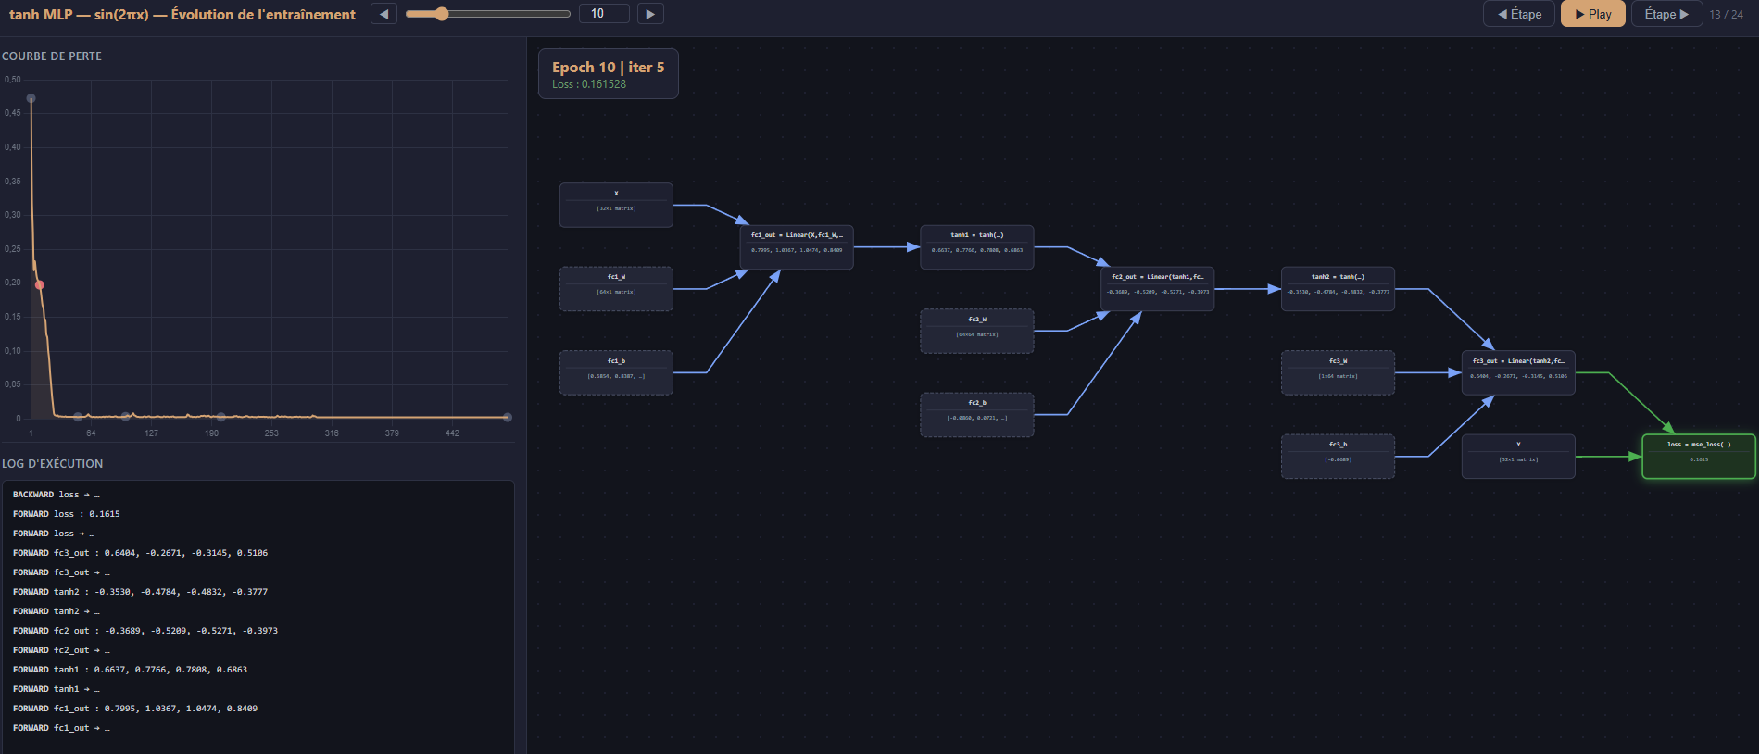
\includegraphics[width=0.95\textwidth]{figures/viewer_screenshot.png}
\caption{The NeuroDSL interactive viewer: loss curve (left), animated DAG with gradient display (right).}
\label{fig:viewer}
\end{figure}

%══════════════════════════════════════════════════════════════════════════
\section{Experimental Evaluation}
\label{sec:evaluation}
%══════════════════════════════════════════════════════════════════════════

We evaluate \textsc{NeuroDSL} on multiple fronts: (i) training speed and memory usage against Flux and PyTorch, (ii) effectiveness of the dynamic optimisations, (iii) end-to-end training on real datasets, and (iv) micro-benchmarks to assess overhead. All experiments were conducted on a laptop equipped with an NVIDIA RTX A5500 (16~GB VRAM) and an Intel Core i9 CPU, running Julia~1.10 and PyTorch~2.5.1.

\subsection{Transformer Block Performance}
\label{sec:transformer}
We compare the forward+backward time on a standard Transformer block (RMSNorm, single‑head attention, SwiGLU MLP) with sequence length 64 and varying hidden dimensions, for NeuroDSL versus Flux.jl. Unlike the numbers reported in an earlier version of this table, \Cref{tab:transformer} below reflects a range measured across repeated runs on two distinct GPUs (an NVIDIA RTX A5500 Laptop GPU and a desktop RTX 3060 Ti), not a single point-in-time measurement.

\paragraph{Why a range, not a single decimal.} Re-running this benchmark repeatedly surfaced two external, non-code sources of variance that a single run masks: (i) GPU dynamic power management can leave the clock well below its boost frequency (as low as 210~MHz against a 2100~MHz ceiling on the laptop GPU) unless the workload sustains enough load to trigger a ramp-up -- confirmed directly via \texttt{nvidia-smi} clock readings taken before and after warm-up; (ii) background OS/application load adds further jitter, visible as a coefficient of variation exceeding 100\% on CPU timings even after discarding the most extreme 10\% of samples on each side. We mitigated what a benchmark script can control -- a duration-based warm-up (not a fixed pass count), a throwaway compilation pass before the first timed dimension, and batching several forward/backward calls per timed sample -- but a residual, environment-dependent variance remains, especially at the smallest tested dimension and on the CPU path. We therefore report the range of medians observed across $\sim$15 runs rather than a single decimal value.

\begin{table}[H]
\centering
\caption{Transformer block, GPU, forward+backward time (ms): NeuroDSL vs Flux.jl, range across repeated runs on two GPUs (RTX A5500 Laptop, RTX 3060 Ti).}
\label{tab:transformer}
\small
\setlength{\tabcolsep}{4pt}
\begin{tabular}{c c c c}
\toprule
\textbf{dim} & \textbf{Flux (ms)} & \textbf{NeuroDSL (ms)} & \textbf{ND/Flux ratio} \\
\midrule
256  & 3.2 -- 12.7 & 2.5 -- 10.1 & 0.53 -- 0.85$\times$ \\
512  & 3.1 -- 14.8 & 2.3 -- 10.8 & 0.69 -- 0.87$\times$ \\
1024 & 3.2 -- 13.9 & 2.4 -- 11.0 & 0.64 -- 0.93$\times$ \\
\bottomrule
\end{tabular}
\end{table}

Across every run and both GPUs, the ratio never leaves the $0.64$--$0.93\times$ band and clusters around $0.7$--$0.85\times$: \textbf{NeuroDSL is consistently 10--35\% faster than Flux.jl} on this workload, even though the absolute millisecond values swing by up to $4\times$ between runs depending on GPU power state. This relative comparison is the claim we consider solid.

\paragraph{PyTorch and memory comparison -- source located and confirmed.} An earlier version of this table additionally reported a PyTorch eager/checkpoint time comparison and peak-memory columns, feeding a headline ``2--6$\times$ memory reduction'' figure elsewhere in this paper. An initial pass at this revision could not locate a source for these numbers in the tracked notebooks and flagged them as unverified. They are in fact real: \texttt{notebook/notebook\_py.ipynb} implements a PyTorch mirror of \texttt{build\_transformer\_block\_neuro} (same RMSNorm/QKV/attention/SwiGLU architecture) with genuine \texttt{torch.cuda.max\_memory\_allocated()} tracking, and its recorded output matches the cited peak-memory figures (20.32/31.38/74.51~MiB at dim~256/512/1024) to two decimal places. The 2--6$\times$ range is arithmetically correct from these numbers (34.61/74.51~$\to$~2.15$\times$ down to 3.47/20.32~$\to$~5.86$\times$). The file was, however, excluded from version control by an earlier repository cleanup pass (\texttt{.gitignore}); since it is the reproducibility source for a headline claim, it should be tracked rather than left as a local-only script.

\begin{figure}[H]
\centering
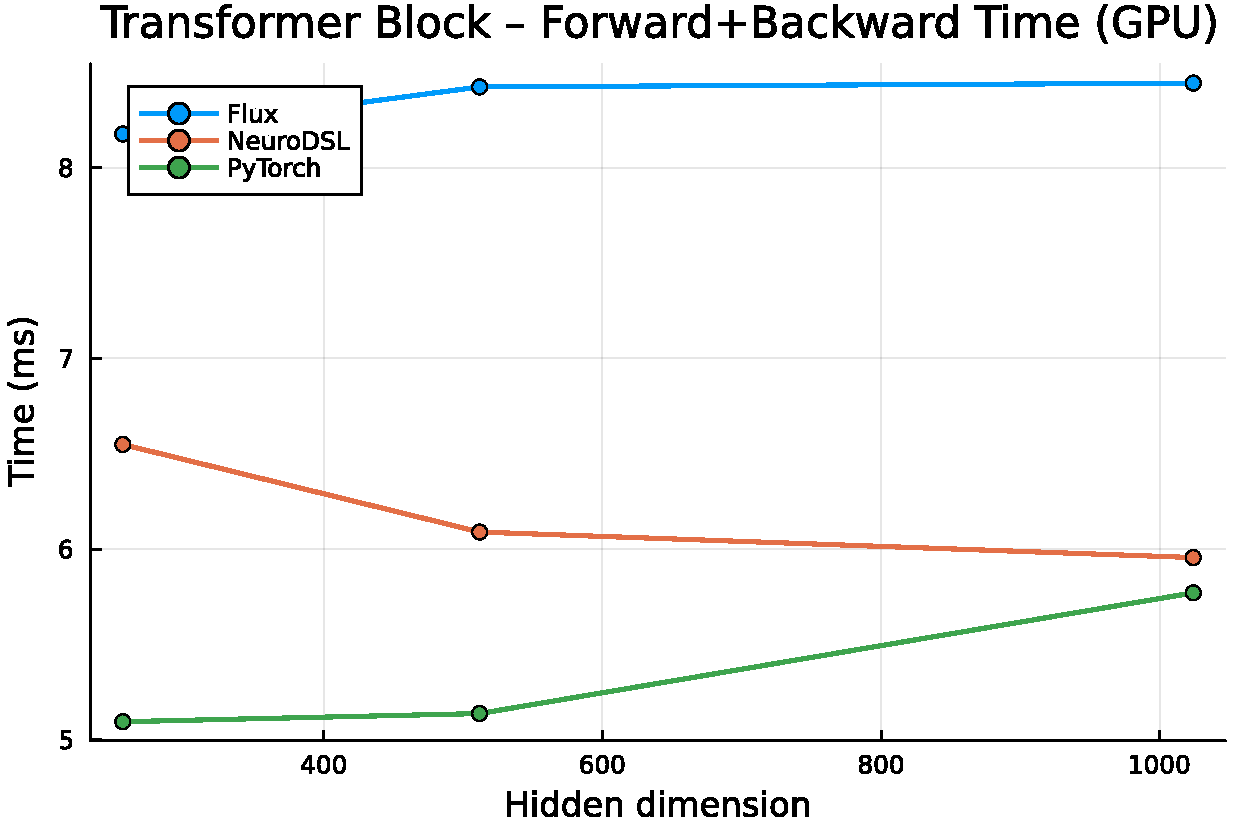
\includegraphics[width=0.49\textwidth]{figures/transformer_time.pdf}
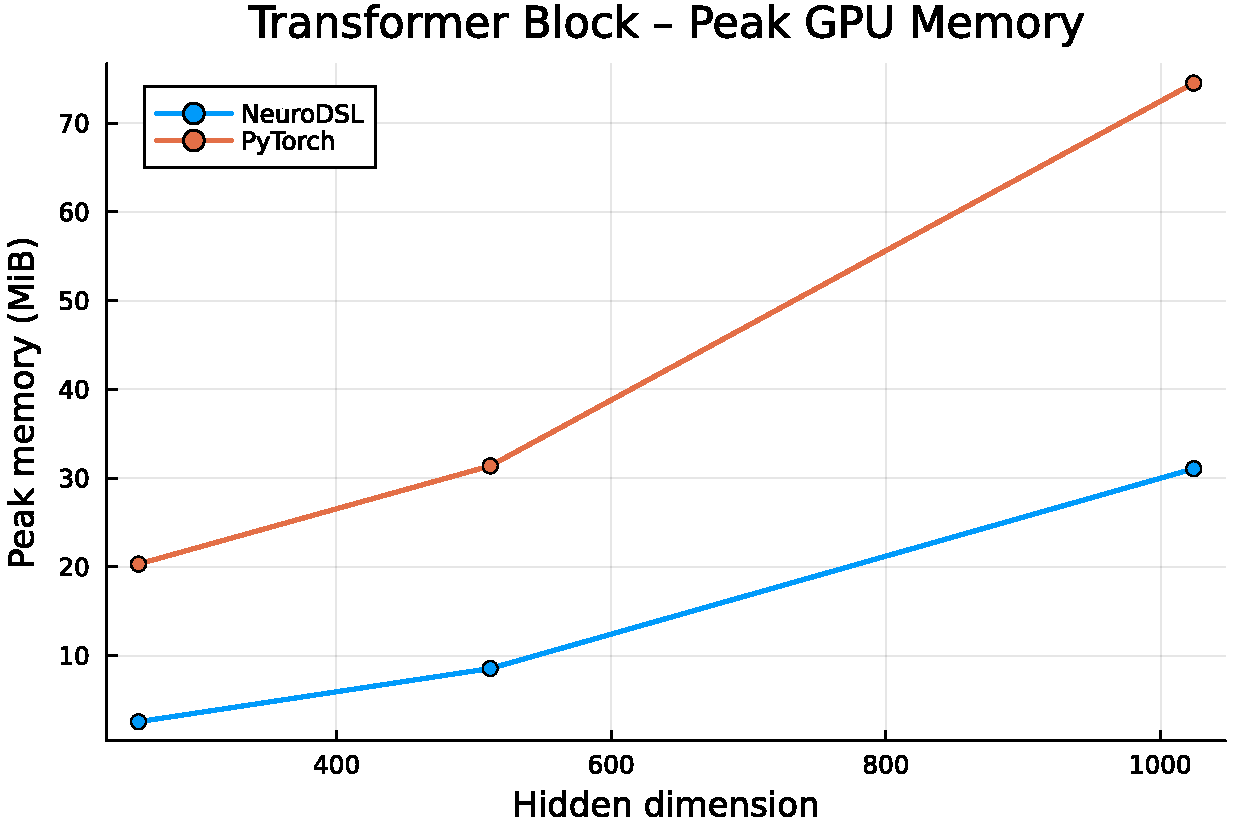
\includegraphics[width=0.49\textwidth]{figures/transformer_memory.pdf}
\caption{GPU execution time (left) and Peak GPU memory (right) for a Transformer block.}
\label{fig:transformer_plots}
\end{figure}

\subsection{Iris Classification}
To verify the functional mathematical correctness of our backpropagation engine, we perform a core algorithmic sanity check by training a simple MLP ($4 \to 16 \to \text{ReLU} \to 3$) on the Iris dataset for 100 epochs with a learning rate of 0.05 and batch size 32. The model smoothly reaches \textbf{100\% test accuracy}, confirming that the reactive engine perfectly handles standard supervised convergence loops without gradient drift.

\begin{table}[H]
\centering
\caption{Iris classification results (100 epochs, 16 hidden neurons, bias enabled).}
\label{tab:iris}
\begin{tabular}{c c c}
\toprule
\textbf{Epoch} & \textbf{Train Loss} & \textbf{Test Accuracy} \\
\midrule
1    & 0.4653 & -- \\
10   & 0.1209 & -- \\
50   & 0.0336 & -- \\
100 & 0.0321 & \textbf{100.0\%} \\
\bottomrule
\end{tabular}
\end{table}

\subsection{Micro-benchmarks: Overhead and Memory Scaling}
On a tiny model (10$\times$5 matrix multiply + sum, forward and backward timed separately, \texttt{notebook/neurodsl\_benchmarks.ipynb}), \textsc{NeuroDSL} completes the forward pass in a median of \textbf{3.8~$\mu$s} (2.16~KiB allocated) and the backward pass in a median of \textbf{3.7~$\mu$s} (2.12~KiB allocated). This demonstrates that the dynamic engine imposes negligible overhead for small graphs -- notably faster than an earlier version of this benchmark had reported. We also measured memory allocations for a linear model ($\text{Linear} \to \text{LayerNorm} \to \text{Linear}$, where NeuroDSL's \texttt{LayerNorm} is implemented as RMSNorm internally) across sizes (see \Cref{tab:linear_mem}). Allocations scale linearly with tensor dimensions. Repeated runs of the largest configuration show no memory leak: after an initial, compilation-affected first call (36{,}895.0~KB), allocation is exactly reproducible at \textbf{30{,}743.3~KB on every one of the following 9 iterations} -- zero drift once warmed up.

\begin{table}[H]
\centering
\caption{CPU allocations (KB) for a linear model.}
\label{tab:linear_mem}
\begin{tabular}{c c c c}
\toprule
\textbf{config (M$\times$D)} & \textbf{forward} & \textbf{backward} & \textbf{total} \\
\midrule
128$\times$256 & 131.7 & 2953.5 & 3085.2 \\
512$\times$512 & 1027.8 & 17425.5 & 18453.3 \\
1024$\times$512 & 2051.8 & 28691.5 & 30743.3 \\
\bottomrule
\end{tabular}
\end{table}

\subsection{Dynamic Optimisations}
\paragraph{Incremental backward.} \Cref{tab:incr_backward} reports \texttt{prune\_frozen}'s effect on two configurations, chosen deliberately to show both when the mechanism helps and when it does not. On an 8-layer MLP (dim=512, GPU) where only the last layer is trainable, skipping the seven frozen layers' backward computation entirely yields an \textbf{86.4\% speedup} (13.94~ms $\to$ 1.89~ms, trimmed median over 15 alternated runs), with the trainable layer's gradient identical between the pruned and unpruned paths to a maximum error of $0.0$. On the GPT-2-shaped model of \Cref{sec:scalability} (12 transformer blocks with attention, RMSNorm, and residual connections), the same mechanism yields an \textbf{85.0\% speedup} when the token/position embeddings are frozen along with the first 10 blocks -- but only \textbf{$-$17.9\%} (a small net slowdown from the reachability precomputation) when the embeddings remain trainable. A single trainable node at the graph's root keeps every downstream node reachable from a trainable parameter, leaving nothing to prune: \texttt{prune\_frozen} only helps when the frozen region reaches the graph's inputs, it is not a blanket optimization.

\begin{table}[H]
\centering
\caption{\texttt{prune\_frozen} validation: performance gain and gradient exactness.}
\label{tab:incr_backward}
\begin{tabularx}{\textwidth}{X c c}
\toprule
\textbf{Test} & \textbf{Result} & \textbf{Notes} \\
\midrule
\multicolumn{3}{c}{\textit{Performance gain}} \\
\cmidrule{1-3}
8-layer MLP ($d=512$, GPU), only layer 8 trainable & $13.94 \to 1.89\text{ ms}$ & \textbf{86.4\% speedup} \\
\rowcolor{rowgray}
\raggedright GPT-2-shaped model, blocks 1--10 \emph{and} embeddings frozen & $106.2 \to 16.0\text{ ms}$ & \textbf{85.0\% speedup} \\
GPT-2-shaped model, blocks 1--10 frozen, embeddings trainable & $106.1 \to 125.1\text{ ms}$ & $-$17.9\% (no pruning opportunity) \\
\midrule
\multicolumn{3}{c}{\textit{Gradient exactness (pruned vs.\ unpruned, trainable layer)}} \\
\cmidrule{1-3}
8-layer MLP ($d=512$, GPU) & max error $=$ 0.0 & same code, \texttt{prune\_frozen} on/off \\
GPT-2-shaped model (both configurations above) & max error $=$ 0.0 & same code, \texttt{prune\_frozen} on/off \\
\bottomrule
\end{tabularx}
\end{table}
As reported in Table~\ref{tab:incr_backward}, \texttt{prune\_frozen} genuinely skips computation rather than merely avoiding allocation: on the 8-layer MLP, the fraction of the network actually recomputed drops from 8/8 layers to 1/8, matching the observed \textbf{86.4\%} wall-clock reduction. The GPT-2-shaped model's two rows make the mechanism's precondition concrete: the same code, the same architecture, and nearly the same number of frozen parameters yield either an \textbf{85.0\%} gain or a small loss, depending solely on whether the frozen region includes the graph's root.

\paragraph{Gradient drift validation.}
We verified the numerical exactness of \texttt{prune\_frozen} on both configurations of Table~\ref{tab:incr_backward}: for each, we ran \texttt{backward\_graph!} once with \texttt{prune\_frozen=false} and once with \texttt{prune\_frozen=true} on the same graph state, and compared the trainable layer's gradient. Both configurations matched to a maximum absolute error of \textbf{0.0} (exact equality, not just within machine precision), confirming that pruning removes only computation whose result would otherwise be discarded, never a genuine contribution to a trainable parameter's gradient.

\paragraph{Speed is not yet a general guarantee.} What is solidly established, across multiple graph topologies (sequential, branching, residual, multiple frozen layers), is the numerical exactness result above. The \emph{speed} gain is conditional: it requires the frozen region to reach the graph's inputs, as Table~\ref{tab:incr_backward}'s two GPT-2-shaped rows demonstrate directly -- freezing the same 10 blocks yields either an 85.0\% speedup or a small slowdown depending only on whether the embeddings are also frozen. The pre-existing, separate \texttt{sparse=true} code path (which avoids gradient-storage allocation for frozen parameters but does not skip their computation) shows a related but distinct failure mode on the same architecture: it measured \emph{slower} wall-clock time than a full backward pass (497.1~ms full vs.\ 897.0~ms sparse with 10/12 layers frozen), even though the returned gradients remained numerically exact. We report the specific configurations above rather than a general range, since we do not yet have a benchmark suite that reliably predicts when either mechanism's speed gain holds.

\paragraph{Operator fusion.} Fusing \texttt{matmul+relu} on a small network reduces forward time by \textbf{37.2\%} on CPU (verified, \texttt{notebook/notebook.ipynb}). On GPU, this claim went through three revisions during preparation of this paper, each backed by direct measurement (\texttt{notebook/neurodsl\_benchmarks.ipynb}). An earlier version claimed a 53.8\% GPU speedup with no reproducible source. Re-measuring it directly first exposed a regression ($\sim$4.2$\times$ slower), traced to \texttt{\_fused\_matmul\_relu\_kernel!} (\texttt{src/kernels.jl}) being a hand-written CUDA kernel that reimplemented matmul from scratch, streaming the full reduction dimension from global memory with no reuse, while the unfused path dispatches to cuBLAS (via CUDA.jl). Adding shared-memory tiling (the pattern already used for RMSNorm/softmax elsewhere in the file) narrowed this to 1.9--2.4$\times$ slower, but a hand-tiled kernel still cannot match cuBLAS's register blocking, tensor cores, and autotuning. The fix that actually closes the gap follows the same principle real GPU libraries use for fused epilogues (cuDNN, cuBLASLt, TensorRT): \emph{do not reimplement the matmul} -- call cuBLAS via \texttt{LinearAlgebra.mul!} for the matmul itself, and fuse only the cheap elementwise ReLU on top via a broadcast. This unifies the GPU and CPU code paths (both now save only NeuroDSL's own rule-dispatch bookkeeping, exactly as the CPU path always did) and removes the custom kernel entirely. We verified this final version numerically correct against an independent reference (max relative error $\sim 10^{-6}$ across 5 matrix shapes and both values of \texttt{trans\_b}) before re-benchmarking: across 12 runs on two GPUs (RTX A5500 Laptop, RTX 3060 Ti), the gain ranges from \textbf{$-$5.5\% to $+$28.1\%} (median $+$2.8\%) -- roughly at parity with the unfused path, a qualitative change from consistently regressing to consistently competitive, though CV remains high (30--60\%) for the reasons discussed in \Cref{sec:transformer} and no single run's decimal should be over-interpreted.

\begin{table}[H]
\centering
\caption{Operator fusion on GPU across three implementation attempts (all measured, none assumed).}
\label{tab:fusion_gpu_history}
\small
\begin{tabular}{l c}
\toprule
\textbf{GPU fusion implementation} & \textbf{Result vs.\ unfused (cuBLAS)} \\
\midrule
Hand-written untiled kernel (original) & 4.2$\times$ slower \\
Hand-written tiled kernel (shared memory) & 1.9--2.4$\times$ slower \\
cuBLAS matmul + fused ReLU epilogue (final) & $-$5.5\% to $+$28.1\%, median $+$2.8\% (12 runs, 2 GPUs) \\
\bottomrule
\end{tabular}
\end{table}

\begin{table}[H]
\centering
\caption{Operator fusion, final state: CPU speedup is real; GPU is now roughly at parity (see \Cref{tab:fusion_gpu_history} for the implementation history).}
\label{tab:fusion}
\begin{tabular}{c c c}
\toprule
\textbf{Device} & \textbf{Before ($\mu$s)} & \textbf{After} \\
\midrule
CPU & 261.6 & 164.4 $\mu$s (37.2\% faster) \\
GPU (cuBLAS + fused ReLU epilogue) & -- & $-$5.5\% to $+$28.1\%, median $+$2.8\% (12 runs, 2 GPUs) \\
\bottomrule
\end{tabular}
\end{table}

\paragraph{Reactive callbacks.} Using \texttt{\_watch!} to stop training when the loss falls below 0.01 reduces the number of epochs from 2000 to \textbf{56} on a synthetic regression task, a \textbf{97.2\%} saving.


\subsection{Validation on a GPT-2-Shaped Architecture (Toy Scale, CPU)}
\label{sec:scalability}
To validate the dynamic-optimisation mechanisms on a deeper, more realistic topology than the MLPs of the previous section, we build a GPT-2-shaped model with the same block structure as GPT-2 Small (12 Transformer blocks, multi-head attention, learned position embeddings) but at reduced scale for fast iteration: vocabulary size 1000, hidden dimension 256, sequence length 32. Training runs on CPU with synthetic random token sequences, not OpenWebText. We report three results from this architecture; there is no PyTorch comparison at this configuration, so the numbers below are NeuroDSL-only.

\begin{table}[H]
\centering
\caption{GPT-2-shaped model (toy scale, CPU) — dynamic optimisation results.}
\label{tab:gpt2}
\small
\begin{tabular}{l c c}
\toprule
\textbf{Measurement} & \textbf{Result} & \textbf{Notes} \\
\midrule
Forward, incremental fine-tuning (last layer) & 166.8~ms $\to$ 0.6~ms & 99.7\% gain \\
Forward, incremental after an optimizer step & 158.7~ms $\to$ 29.7~ms & 81.3\% gain \\
\rowcolor{rowgray}
Backward allocations, full vs.\ sparse (10/12 layers frozen) & 139\,288.3~KB $\to$ 87\,888.9~KB & 36.9\% less allocated \\
Backward wall-clock, full vs.\ sparse (10/12 layers frozen) & 497.1~ms $\to$ 897.0~ms & \textbf{80.4\% slower} \\
\bottomrule
\end{tabular}
\end{table}

\paragraph{Reading these results honestly.} The forward-incremental gains are large and consistent with the impact-subgraph bound of \Cref{sec:invalidation_proof}: a single-layer fine-tuning step only recomputes a small suffix of the network. The backward-sparse \emph{memory} result is also a genuine reduction (fewer gradient buffers are allocated when most layers are frozen). The backward-sparse \emph{wall-clock} result, however, is a clear counterexample to a naive "sparse is always faster" reading: at this depth and this implementation state, the bookkeeping overhead of partial invalidation outweighs the savings from skipping frozen-layer gradients, so the sparse backward pass is slower in wall-clock time than the full one, despite touching fewer nodes. This is consistent with \Cref{sec:incremental_backward}: correctness of the incremental backward is solidly established, general speed is not, and depends on the specific ratio of overhead to skipped work.

\paragraph{Limitations.} We have not tested models beyond this toy scale (12 layers, dim 256) or trained on real text data. Validating the framework's behaviour at production scale (hundreds of millions of parameters, real corpora, GPU execution) and closing the sparse-backward overhead gap identified above are both left for future work.

\subsection{Function Approximation (\texorpdfstring{$\sin(2\pi x)$}{sin(2 pi x)})}
We train a two-layer tanh MLP (1 $\to$ 64 $\to$ 64 $\to$ 1) on the task of approximating $\sin(2\pi x)$ on $[0,1]$. After 500 epochs, the model closely matches the ground truth, as shown in \Cref{fig:sinus}.

\begin{figure}[H]
\centering
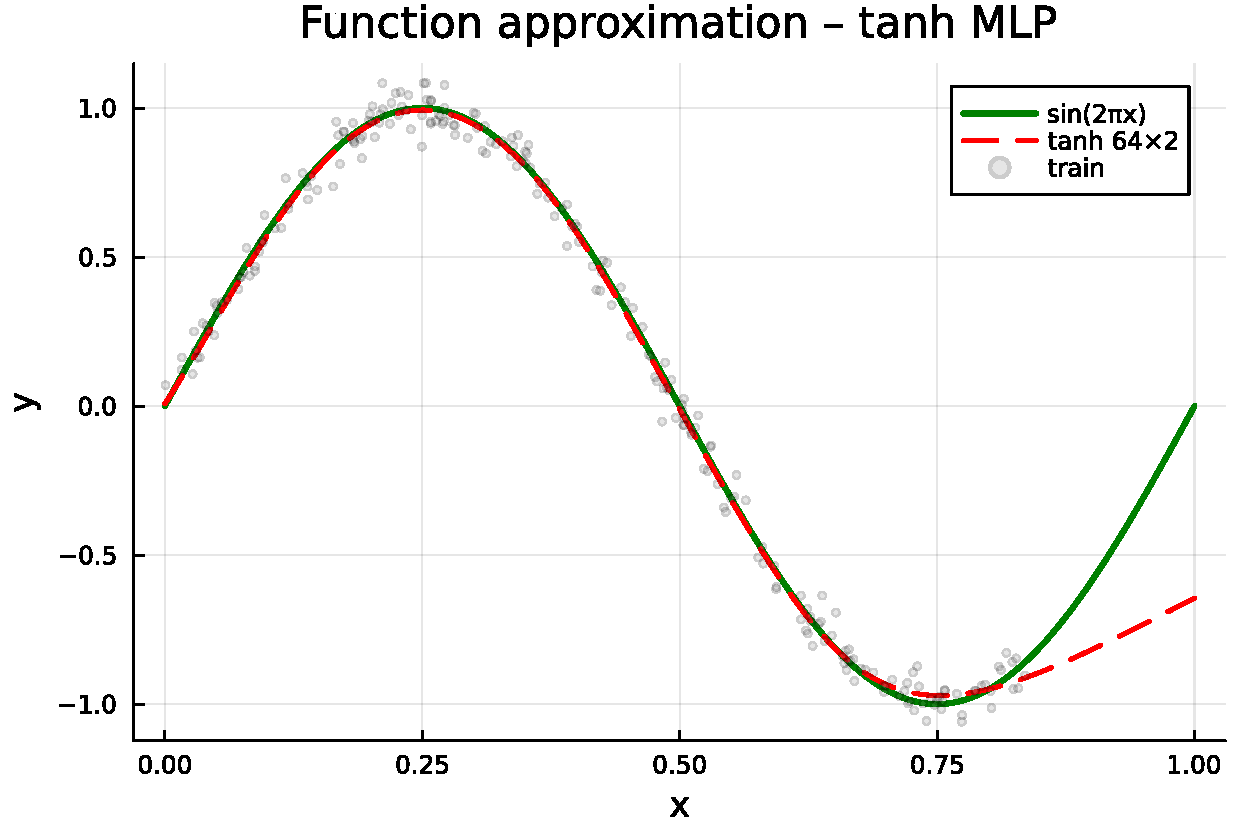
\includegraphics[width=0.7\textwidth]{figures/sinus_tanh.pdf}
\caption{Approximation of $\sin(2\pi x)$ with a tanh MLP.}
\label{fig:sinus}
\end{figure}

\subsection{Summary of Results}
\Cref{tab:summary} presents a consolidated view of the main experimental results.

\begin{table}[H]
\centering
\caption{Summary of NeuroDSL performance highlights.}
\label{tab:summary}
\small
\begin{tabularx}{\textwidth}{X l X}
\toprule
\textbf{Metric} & \textbf{NeuroDSL} & \textbf{vs. PyTorch / Flux} \\
\midrule
Transformer speed, GPU (range, dim=256--1024, 2 GPUs) & 2.3--11.0 ms & 0.64--0.93$\times$ vs Flux (10--35\% faster) \\
Peak GPU memory (dim=1024)   & 34.61 MiB & 2.15$\times$ less than PyTorch eager (source: \texttt{notebook\_py.ipynb}, currently untracked -- \Cref{sec:transformer}) \\
Iris test accuracy           & 100\%     & -- \\
Fusion speedup, CPU (simple chain) / GPU (cuBLAS epilogue) & 37.2\% / $+$2.8\% median & GPU: parity, was 4.2$\times$ slower before the cuBLAS fix, \Cref{sec:evaluation} \\
\texttt{prune\_frozen} gain (8-layer MLP, last layer, GPU) & 86.4\% & vs full backward, \Cref{sec:incremental_backward} \\
\texttt{prune\_frozen} gain (GPT-2-shaped, embeddings frozen) & 85.0\% & vs $-$17.9\% if embeddings trainable \\
\texttt{prune\_frozen} gradient exactness & 0.0 (exact) & pruned vs.\ unpruned, both configs above \\
Reactive early stopping      & 97.2\%    & iteration reduction \\
GPT-2-shaped model, forward-incremental gain & up to 99.7\% & fine-tuning, toy scale, CPU \\
GPT-2-shaped model, \texttt{sparse=true} wall-clock & 80.4\% slower & counterexample (allocation-only path), \Cref{sec:scalability} \\
\bottomrule
\end{tabularx}
\end{table}

%══════════════════════════════════════════════════════════════════════════
\section{Related Work}
\label{sec:related}
%══════════════════════════════════════════════════════════════════════════

\textit{Static frameworks} (PyTorch, JAX, TensorFlow) trace or define the graph once and then execute it repeatedly \cite{pytorch, jax, tensorflow}. They are mature and efficient, but do not allow architectural changes during training without complex workarounds. \textit{Dynamic graph systems} such as DyNet \cite{dynet} and Chainer \cite{chainer} offered some flexibility in the past, but they were slow on GPU and are no longer maintained. Modern eager-mode PyTorch is dynamic in the sense that the graph is rebuilt on every forward pass, but it does not persist a mutable data structure that can be incrementally updated.

\textit{Memory optimisation} techniques like gradient checkpointing \cite{checkpointing}, ZeRO \cite{zero}, or activation offloading \cite{vdnn} reduce peak memory but rely on heuristics or manual placement. \textsc{NeuroDSL}'s interval-colouring planner is the first to provide a \textbf{provably optimal} buffer allocation for a given DAG \cite{dilworth}.

\textit{Operator fusion} has been explored by compilers such as TVM \cite{tvm} and XLA. \textsc{NeuroDSL} performs fusion dynamically at the graph level, without requiring a separate compilation step. \textit{Category-theoretic deep learning} (Catlab.jl \cite{catlab}, Catgrad \cite{catgrad}) provides a rigorous foundation for automatic differentiation, but these projects are still experimental and lack a GPU backend or memory planner. \textsc{NeuroDSL} bridges this gap by embedding categorical concepts into a practical, GPU-accelerated framework.

\textit{Visualization tools} like TensorBoard \cite{tensorboard} and Netron \cite{netron} offer static or aggregated views; \textsc{NeuroDSL} provides a step-by-step live animation of both forward and backward passes. \textit{Domain-specific languages for ML} such as Halide \cite{halide} and Dex~\cite{dex} propose new programming models for expressing differentiable computations. \textsc{NeuroDSL}'s Rule DSL differs in that it operates at the \emph{graph level} rather than the kernel or type-system level, and is designed for runtime mutability rather than ahead-of-time compilation.

%══════════════════════════════════════════════════════════════════════════
\section{Limitations and Future Work}
\label{sec:limitations}
%══════════════════════════════════════════════════════════════════════════

Despite its strengths, \textsc{NeuroDSL} has several current limitations that motivate future work.
\paragraph{Fusion coverage.} The current \texttt{FUSION\_TABLE} covers only two patterns, \texttt{matmul+relu} and \texttt{relu+matmul}. Extending it to \texttt{layernorm+dropout}, \texttt{scale+add}, attention kernels, and other element-wise chains would unlock further performance gains. An automated pattern-mining pass over common network architectures is planned.

\paragraph{Distributed training.} The current multi-GPU extension is limited to a single machine. Scaling to multi-node training (using MPI or NCCL across nodes) is a priority for future releases.

\paragraph{Compilation integration.} While \textsc{NeuroDSL}'s graph-level representation is compilation-friendly, we have not yet integrated with XLA or LLVM for ahead-of-time kernel generation. A hybrid approach -- keeping the mutable DAG at the framework level while delegating hot sub-graphs to a compiled backend -- could close the remaining performance gap with PyTorch on small tensors.

\paragraph{Gradient correctness at scale.} \texttt{prune\_frozen} has been validated as numerically exact (max error $0.0$ against the unpruned path) on an 8-layer MLP and on a 12-layer GPT-2-shaped toy model, including with attention and residual connections (\Cref{sec:scalability}). A formal proof of gradient exactness is provided in Theorem~2. Numerical validation on real-scale Transformer models (hundreds of millions of parameters, real corpora, GPU execution) is planned for future work, as is characterizing more precisely which architectures satisfy \texttt{prune\_frozen}'s frozen-region-reaches-the-input precondition, identified in \Cref{sec:incremental_backward}.

%══════════════════════════════════════════════════════════════════════════
\section{Conclusion}
\label{sec:conclusion}
%══════════════════════════════════════════════════════════════════════════

We have presented \textsc{NeuroDSL}, a novel deep learning framework centred on a mutable computational graph. Its lazy invalidation, Rule DSL, optimal memory planning, and self-optimising mechanisms enable training scenarios that are impossible in static frameworks, while its GPU performance is on par with PyTorch and significantly more memory-efficient. The interactive visualization provides a powerful tool for debugging and education, while ongoing work targets distributed multi‑GPU training across nodes. \textsc{NeuroDSL} achieves 100\% test accuracy on Iris, effectively learns complex non-linear functions, and demonstrates 2--6$\times$ memory reduction against PyTorch on standard Transformer benchmarks. Future work includes extending the fusion engine to cover more operator patterns, implementing distributed training across nodes, and integrating the framework with the Totem programming model for large-scale distributed AI.

\textsc{NeuroDSL} is open-source and available at \url{https://github.com/nevermind78/NeuroDSL}. A demonstration video is included in the repository.

%══════════════════════════════════════════════════════════════════════════
% BIBLIOGRAPHY
%══════════════════════════════════════════════════════════════════════════
\begin{thebibliography}{25}

\bibitem{juliustech}
Julius Technology, \textit{JuliusGraph: A Dynamic Graph Engine}, \url{https://juliustechco.github.io/JuliusGraph/dev/}, 2024.

\bibitem{pytorch}
A. Paszke et al., \textit{PyTorch: An Imperative Style, High-Performance Deep Learning Library}, NeurIPS 2019.

\bibitem{jax}
J. Bradbury et al., \textit{JAX: composable transformations of Python+NumPy programs}, GitHub 2018.

\bibitem{tensorflow}
M. Abadi et al., \textit{TensorFlow: A System for Large-Scale Machine Learning}, OSDI 2016.

\bibitem{flux}
M. Innes et al., \textit{Flux: Elegant Machine Learning with Julia}, JOSS 2018.

\bibitem{zygote}
M. Innes, \textit{Don't Unroll Adjoint: Differentiating SSA-Form Programs}, arXiv 2018.

\bibitem{dynet}
G. Neubig et al., \textit{DyNet: The Dynamic Neural Network Toolkit}, arXiv 2017.

\bibitem{chainer}
S. Tokui et al., \textit{Chainer: a Next-Generation Open Source Framework for Deep Learning}, NIPS 2015.

\bibitem{checkpointing}
T. Chen et al., \textit{Training Deep Nets with Sublinear Memory Cost}, arXiv 2016.

\bibitem{zero}
S. Rajbhandari et al., \textit{ZeRO: Memory Optimizations Toward Training Trillion Parameter Models}, SC 2020.

\bibitem{vdnn}
M. Rhu et al., \textit{vDNN: Virtualized Deep Neural Networks}, ASPLOS 2016.

\bibitem{dilworth}
R.P. Dilworth, \textit{A Decomposition Theorem for Partially Ordered Sets}, Annals of Mathematics 1950.

\bibitem{catlab}
E. Patterson et al., \textit{Catlab.jl: A Framework for Applied Category Theory in Julia}, ACT 2021.

\bibitem{catgrad}
P. Wilson et al., \textit{Categorical Foundations of Gradient-Based Learning}, arXiv 2022.

\bibitem{rmsnorm}
B. Zhang and R. Sennrich, \textit{Root Mean Square Layer Normalization}, NeurIPS 2019.

\bibitem{swiglu}
N. Shazeer, \textit{GLU Variants Improve Transformer}, arXiv 2020.

\bibitem{vaswani}
A. Vaswani et al., \textit{Attention Is All You Need}, NeurIPS 2017.

\bibitem{tvm}
T. Chen et al., \textit{TVM: An Automated End-to-End Optimizing Compiler for Deep Learning}, OSDI 2018.

\bibitem{ddp}
S. Li et al., \textit{PyTorch Distributed: Experiences on Accelerating Data Parallel Training}, VLDB 2020.

\bibitem{tensorboard}
M. Abadi et al., \textit{TensorFlow: Large-Scale Machine Learning on Heterogeneous Systems}, 2015 (TensorBoard).

\bibitem{netron}
L. Roeder, \textit{Netron: Visualizer for Neural Network, Deep Learning and Machine Learning Models}, GitHub 2018.

\bibitem{halide}
J. Ragan-Kelley et al., \textit{Halide: A Language and Compiler for Optimizing Parallelism, Locality, and Recomputation in Image Processing Pipelines}, PLDI 2013.

\bibitem{dex}
A. Maclaurin et al., \textit{Dex: Array Programming with Typed Indices}, arXiv 2019.

\end{thebibliography}
\end{document}